\documentclass[10pt,twocolumn]{article}
\usepackage[margin=0.65in]{geometry}
\usepackage{graphicx}
\usepackage{booktabs}
\usepackage{array}
\usepackage{amsmath}
\usepackage{cite}
\usepackage{hyperref}
\usepackage{microtype}

\renewcommand{\topfraction}{0.92}
\renewcommand{\dbltopfraction}{0.92}
\renewcommand{\textfraction}{0.07}
\renewcommand{\floatpagefraction}{0.85}
\renewcommand{\dblfloatpagefraction}{0.85}

\graphicspath{{../figures/}{figures/}}

\title{\textbf{Lineage-Restricted Transcriptomic Prognosis and Normoxic Pharmacogenomic Uncoupling of the \textit{SMARCA4}--\textit{HIF1A} Axis Across Solid Tumors}}
\author{Sachsin Sinnathurai\\
Department of Anatomy \& Cell Biology, McGill University, Montreal, QC, Canada\\
\texttt{sachsin.sinnathurai@mail.mcgill.ca}}
\date{November 2026}

\begin{document}
\raggedbottom
\setlength{\abovedisplayskip}{5pt plus 1pt minus 1pt}
\setlength{\belowdisplayskip}{5pt plus 1pt minus 1pt}
\setlength{\abovedisplayshortskip}{3pt}
\setlength{\belowdisplayshortskip}{3pt}
\maketitle

\begin{abstract}
Hypoxic solid tumors coordinate chromatin remodeling and amino acid transport to sustain growth under therapeutic stress, yet standard functional genomics screens operate in ambient $21\%\ \text{O}_2$ air. Across Broad DepMap 24Q2 CRISPR-Cas9 Chronos profiles of $1,038$ solid tumor lines, the amino acid transporters \textit{SLC1A5} and \textit{SLC7A1} shared positive essentiality ($r = +0.207$, $p = 1.51 \times 10^{-11}$). Physiological \textit{HIF1A}--\textit{SLC7A1} mRNA correlation was similarly strong across $1,384$ primary TCGA tumors ($r = +0.2844$, $p = 3.72 \times 10^{-27}$), but disappeared in normoxic $21\%\ \text{O}_2$ solid cell lines ($r = +0.0249$, $p = 0.360$). Only \textit{VHL} loss-of-function lines ($n = 19$) with constitutive hypoxia signaling preserved \textit{HIF1A}--\textit{SLC7A1} Chronos dependency coupling ($r = +0.5412$, Spearman $\rho = +0.5439$). Across four NCBI GEO $1\%\ \text{O}_2$ hypoxia series, \textit{CA9} and \textit{VEGFA} rose consistently while \textit{HIF1A} mRNA stayed flat or fell. Acute hypoxia failed to induce \textit{SLC7A1} in three models and raised it only transiently at 24~h in HepG2 before reversing by day~6. In unpaired ChIP-Atlas tracks, constitutive \textit{SMARCA4} occupancy in \textit{HIF1A}-null 786-O cells overlapped hypoxic \textit{HIF1A} binding at an intronic \textit{SLC7A1} enhancer in RCC4+\textit{VHL}. Clinically, an unweighted a priori \textit{SMARCA4} + \textit{HIF1A} score stratified overall survival across $5,102$ tumors in 10 primary cohorts ($\text{HR}^* = 1.144$, $p = 9.10 \times 10^{-8}$) and eight non-breast primary cohorts ($\text{HR}^* = 1.152$, $p = 7.27 \times 10^{-5}$). Single-gene decomposition showed that \textit{SMARCA4} carried most of this hazard ($\text{HR}^* = 1.153$, $p = 2.82 \times 10^{-4}$), whereas \textit{HIF1A} mRNA alone was null ($\text{HR}^* = 1.047$, $p = 0.222$). Complete 10-cohort \textit{MKI67} proliferation adjustment incorporating the full $24,326$-gene CGGA-325 transcriptome attenuated pooled risk to $\text{HR}^* = 1.084$ ($p = 0.004$) and abolished glioma stratification ($\text{HR} = 1.006$, $p = 0.943$). Across all 19 solid TCGA cohorts ($N = 7,875$), the two-gene score became null ($\text{HR}^* = 1.048$, $p = 0.130$), while the 14-gene non-cell-cycle \textit{Buffa-14} hypoxia signature stayed strongly prognostic ($\text{HR}^* = 1.133$, $p = 2.17 \times 10^{-6}$). Independent \textit{SMARCA4} + \textit{HIF1A} risk therefore localized strictly to clear cell renal and urothelial bladder carcinomas. In normoxic Sanger GDSC2 $1 - \text{AUC}$ screens ($m = 286$ drugs), only Navitoclax cleared 5\% FDR ($q = 0.049$, partial $R^2 = 2.45\%$) and nine compounds cleared 10\% FDR ($\eta_p^2 = 1.55\%\text{--}2.63\%$), whereas TOP1 and PARP1/2 trends faded after \textit{MKI67} control and $0/3$ combinations tracked baseline risk. Lineage-independent \textit{SLFN11} and \textit{BAK1} gates remained intact on both $1 - \text{AUC}$ and $\ln(\text{IC}_{50})$. Harmonized UCSC Xena Toil comparisons against GTEx v6 showed high normal cardiac ($44.08\text{--}59.22$ TPM) and hepatic ($67.54$ TPM) \textit{MCL1} relative to solid tumors ($114.25$ TPM), pointing toward tumor-targeted delivery and physiological hypoxia models while public human AZD5991 pharmacokinetics remain incomplete.
\end{abstract}

\section{Introduction}
Solid tumors exposed to chronic hypoxia remodel chromatin accessibility, amino acid transport, and drug efflux pathways to survive cytotoxic stress. Under normoxia, prolyl hydroxylases (PHD1--3) hydroxylate hypoxia-inducible factor 1-alpha (HIF-1$\alpha$), targeting the protein for von Hippel--Lindau (VHL) E3 ubiquitin ligase-mediated proteasomal degradation \cite{ivan2001,jaakkola2001}. Hypoxia inhibits PHD1--3 and stabilizes HIF-1$\alpha$ post-translationally, enabling transcriptional cooperation with the mammalian SWI/SNF (BAF) ATPase subunit \textit{SMARCA4} (BRG1) \cite{kenneth2009,sena2013}. Downstream metabolic and survival programs elevate the cationic amino acid uniporter \textit{SLC7A1} (CAT-1), the neutral amino acid antiporter \textit{SLC1A5} (ASCT2), and the multidrug efflux pump \textit{ABCB1} (MDR1). Routine monolayer CRISPR and drug screens grown in ambient $21\%\ \text{O}_2$ air maintain PHD1--3/VHL-mediated HIF-1$\alpha$ turnover and suppress hypoxic signaling, obscuring how apical chromatin and hypoxia regulators relate to amino acid transporters and clinical outcomes in vivo.

To bridge in vitro dependency screens with patient tumor biology, we integrated Broad DepMap 24Q2 CRISPR-Cas9 Chronos profiles across $1,038$ solid tumor lines and $1,719$ unique expression models \cite{depmap2021} with multivariable survival modeling. Our clinical survival analysis covered $5,102$ complete-case solid tumors across 10 primary cohorts ($2,162$ deaths), an independent pancreatic validation cohort in ICGC/PCAWG-PAAD ($N = 71$, 48 deaths), and an expanded 19-cohort solid TCGA benchmark ($N = 7,875$) \cite{tcga2018,cgga2021,curtis2012,raphael2017}. We also tested hypoxic transcriptional responses directly across four paired $1\%$ versus $21\%\ \text{O}_2$ NCBI GEO series (\texttt{GSE283995}, \texttt{GSE139673}, \texttt{GSE145108}, and \texttt{GSE300765}) and nine solid-tumor ChIP-Atlas \textit{HIF1A} and \textit{SMARCA4} tracks at \textit{SLC7A1}. Finally, we evaluated cell-type specificity, pathway activity, pharmacogenomic sensitivity, and normal-organ expression using paired PDAC single-cell RNA-seq from \texttt{CRA001160} \cite{peng2019,han2023}, MSigDB v2024.1 Hallmark gene sets \cite{liberzon2015}, TCPA Level-4 RPPA proteomics \cite{li2013,akbani2014}, TCGA chromosomal instability scores \cite{knijnenburg2018}, IMvigor210 anti-PD-L1 survival ($N = 347$) \cite{mariathasan2018}, Sanger GDSC2 monotherapy and combination screens \cite{jaaks2022,bashi2024}, harmonized UCSC Xena Toil TCGA versus GTEx v6 expression \cite{vivian2017}, and Phase~I pharmacokinetic benchmarks \cite{hamilton2023,desai2024}.

\section{Results}

\subsection{Solute Carrier Co-Dependency, Core BAF Co-Essentiality, and Normoxic Uncoupling}
We first asked whether amino acid transporters linked to hypoxic survival show coordinated functional essentiality in cultured solid tumor lines. Across $1,038$ solid tumor cell lines in Broad DepMap 24Q2, CRISPR-Cas9 Chronos dependency on \textit{SLC1A5} correlated positively with \textit{SLC7A1} ($r = +0.207$, $p = 1.51 \times 10^{-11}$; Figure~1A), clearing Benjamini-Hochberg correction across 10 candidate pairs ($q = 1.51 \times 10^{-10}$). Across all $1,186$ pan-cancer CRISPR-screened lines, \textit{SLC7A1} dependency also tracked with the neutral and branched-chain transporter \textit{SLC7A5} ($r = +0.4024$, $p = 2.23 \times 10^{-47}$; solid-only $r = +0.3882$). Neither gene correlated with its closest paralog: \textit{SLC7A1} was independent of \textit{SLC7A2} ($r = +0.0110$, $p = 0.705$), and \textit{SLC1A5} was independent of \textit{SLC1A4} ($r = -0.0155$, $p = 0.593$). To define the chromatin remodeling partners of \textit{SMARCA4}, we scanned $18,434$ genes comparing \textit{SMARCA4}-dependent solid lines ($n = 299$, $\text{Chronos} \le -0.50$) against independent lines ($n = 251$, $\text{Chronos} \ge -0.10$). Dependent lines required core BAF subunits led by \textit{SMARCB1} ($\Delta = -0.307$, $p = 3.04 \times 10^{-17}$, $q = 5.61 \times 10^{-13}$), \textit{SMARCC1}, \textit{SMARCD1}, \textit{ARID1A}, \textit{SMARCE1}, and \textit{MLLT1} ($p = 8.30 \times 10^{-17}$ to $1.57 \times 10^{-7}$). Continuous \textit{SMARCA4} and \textit{SMARCB1} Chronos scores tracked closely across all $1,038$ solid lines ($r = +0.295$, $\rho = +0.304$). Conversely, \textit{SMARCA4} dependence coincided with synthetic-lethal paralog buffering by \textit{SMARCA2} ($\Delta = +0.133$, $p = 1.32 \times 10^{-8}$, $q = 1.93 \times 10^{-5}$; continuous $r = -0.197$; Figure~1B). Non-malignant diploid fibroblast and epithelial lines ($n = 16$) exhibited substantially weaker single-gene \textit{SMARCA4} dependency than solid tumor lines ($\Delta_{\text{mean}} = +0.260$, $\Delta_{\text{median}} = +0.205$, Mann-Whitney $p = 0.007$; Figure~1C).

We next tested whether ambient $21\%\ \text{O}_2$ culture disrupts transcriptional coupling between \textit{HIF1A} and \textit{SLC7A1}. Across $1,384$ primary tumors from TCGA-PAAD ($n = 176$), TCGA-GBM ($n = 158$), and TCGA-BRCA ($n = 1,050$), within-cohort Z-scored \textit{HIF1A} and \textit{SLC7A1} mRNA levels correlated robustly ($r = +0.2844$, $p = 3.72 \times 10^{-27}$; raw $r = +0.3651$). In normoxic DepMap solid cultures ($n = 1,349$ unique lines standardized within lineage), that correlation collapsed ($r = +0.0249$, $p = 0.360$; Fisher $Z = 6.98$, $p = 2.87 \times 10^{-12}$; Figure~1D). Unadjusted DepMap profiles gave identical null results across $1,719$ unique models ($r = +0.0242$) and $1,775$ total profiles ($r = +0.0185$). Restricting DepMap to Pancreas, CNS/Brain, and Breast models retained modest co-expression ($n = 229$ unique lines, $r = +0.2154$, $p = 0.001$; $n = 221$ solid lines, $r = +0.1736$), even as pan-cancer coupling broke down globally. When we isolated the 19 solid lines carrying truncating or splice loss-of-function \textit{VHL} mutations---predominantly \textit{EPAS1}-dependent ccRCC models---constitutive hypoxia signaling preserved \textit{HIF1A}--\textit{SLC7A1} Chronos dependency coupling ($r = +0.5412$, $p = 0.017$; Spearman $\rho = +0.5439$, $p = 0.016$). Leave-one-out deletion confirmed that no single \textit{VHL}-mutant line drove this correlation, while the $1,019$ wild-type solid lines remained null ($r = -0.0336$, $p = 0.284$). Those 19 \textit{VHL}-deficient lines also showed selective \textit{EPAS1} vulnerability (mean Chronos $-0.3464$ vs.\ $+0.0045$ in pan-solid WT, $d = -2.644$, Welch $p = 0.001$) relative to wild-type kidney ($n = 15$, $p = 6.74 \times 10^{-4}$) and non-ccRCC wild-type models ($n = 1,018$, $p = 1.15 \times 10^{-3}$), whereas wild-type kidney lines matched extra-renal models ($p = 0.372$).

To check whether hypoxic exposure alone restores \textit{HIF1A} and \textit{SLC7A1} transcription in vitro, we analyzed four paired $1\%$ versus $21\%\ \text{O}_2$ NCBI GEO series and nine ChIP-Atlas tracks. Canonical targets \textit{CA9} ($\log_2\text{FC} = +3.079$ to $+4.982$, $p \le 9.54 \times 10^{-4}$) and \textit{VEGFA} ($+0.968$ to $+1.813$, $p \le 0.009$) rose strongly across all four studies: HepG2 liver carcinoma (\texttt{GSE283995}, $n = 6$ per arm at 24~h), AsPC-1 PDAC (\texttt{GSE139673}, $n = 3$ pairs at 24~h), pooled RKO/A549/H460 lines (\texttt{GSE145108}, $n = 6$ pairs at 24~h), and U87MG glioblastoma (\texttt{GSE300765}, $n = 3$ pairs at 48~h). Silencing \textit{ARNT} in hypoxic AsPC-1 reversed \textit{CA9} induction by $-1.967$ $\log_2$-units ($p = 0.012$), verifying functional HIF pathway activation. By contrast, \textit{HIF1A} mRNA failed to rise in every dataset ($\log_2\text{FC} = -1.111$ to $+0.107$), consistent with post-translational protein stabilization. Moreover, 24--48~h hypoxia failed to elevate \textit{SLC7A1} in three of the four models. \textit{SLC7A1} stayed flat in U87MG ($p = 0.517$) and declined in AsPC-1 ($\log_2\text{FC} = -0.458$, $p = 0.001$) and pooled RKO/A549/H460 ($-0.779$, $p = 0.028$) alongside lower \textit{SMARCA4} mRNA ($-0.235$ to $-0.563$). Within \texttt{GSE145108} ($n = 2$ pairs per line), \textit{SLC7A1} shifted downward in RKO ($-0.254$, $p = 0.181$), A549 ($-0.716$, $p = 0.437$), and H460 ($-1.367$, $p = 0.009$). In HepG2, an initial 24-hour rise in \textit{SLC7A1} ($\log_2\text{FC} = +0.299$, $p = 4.78 \times 10^{-5}$) and \textit{SLC1A5} ($+0.128$, $p = 0.008$) reversed after 6~days of chronic $1\%\ \text{O}_2$ hypoxia ($n = 5$), leaving \textit{SLC7A1} below normoxia ($-0.200$, $p = 0.121$) and \textit{SLC1A5} near baseline ($+0.107$, $p = 0.382$) even while \textit{CA9} ($+3.376$, $p = 4.99 \times 10^{-6}$) and \textit{VEGFA} ($+0.775$) stayed induced alongside higher \textit{SMARCA4} ($+0.356$, $p = 0.011$). At the chromatin level, unpaired ChIP-Atlas tracks (MACS2 $q < 10^{-5}$) revealed 19 overlapping \textit{HIF1A} and \textit{SMARCA4} peak pairs across the \textit{SLC7A1} promoter and first intron (\texttt{chr13:29,500,000--29,620,000}) alongside 19 pairs at \textit{VEGFA}. Because 786-O ccRCC cells lack functional \textit{HIF1A} and signal through \textit{EPAS1}, strong \textit{SMARCA4} binding at the \textit{SLC7A1} intronic enhancer (\texttt{SRX8566545}, MACS2 score $493$, $7.08\times$ enrichment) reflects constitutive SWI/SNF bookmarking independent of \textit{HIF1A}. That exact $443\text{ bp}$ element overlapped the hypoxic \textit{HIF1A} peak in \textit{HIF1A}-intact RCC4+\textit{VHL} cells (\texttt{SRX15691692}, MACS2 score $373$, $11.18\times$). Similar overlaps appeared in melanoma, breast, and prostate lines, though paired co-ChIP in matched hypoxic cells is still needed to establish simultaneous co-occupancy.

\begin{figure*}[!t]
\centering
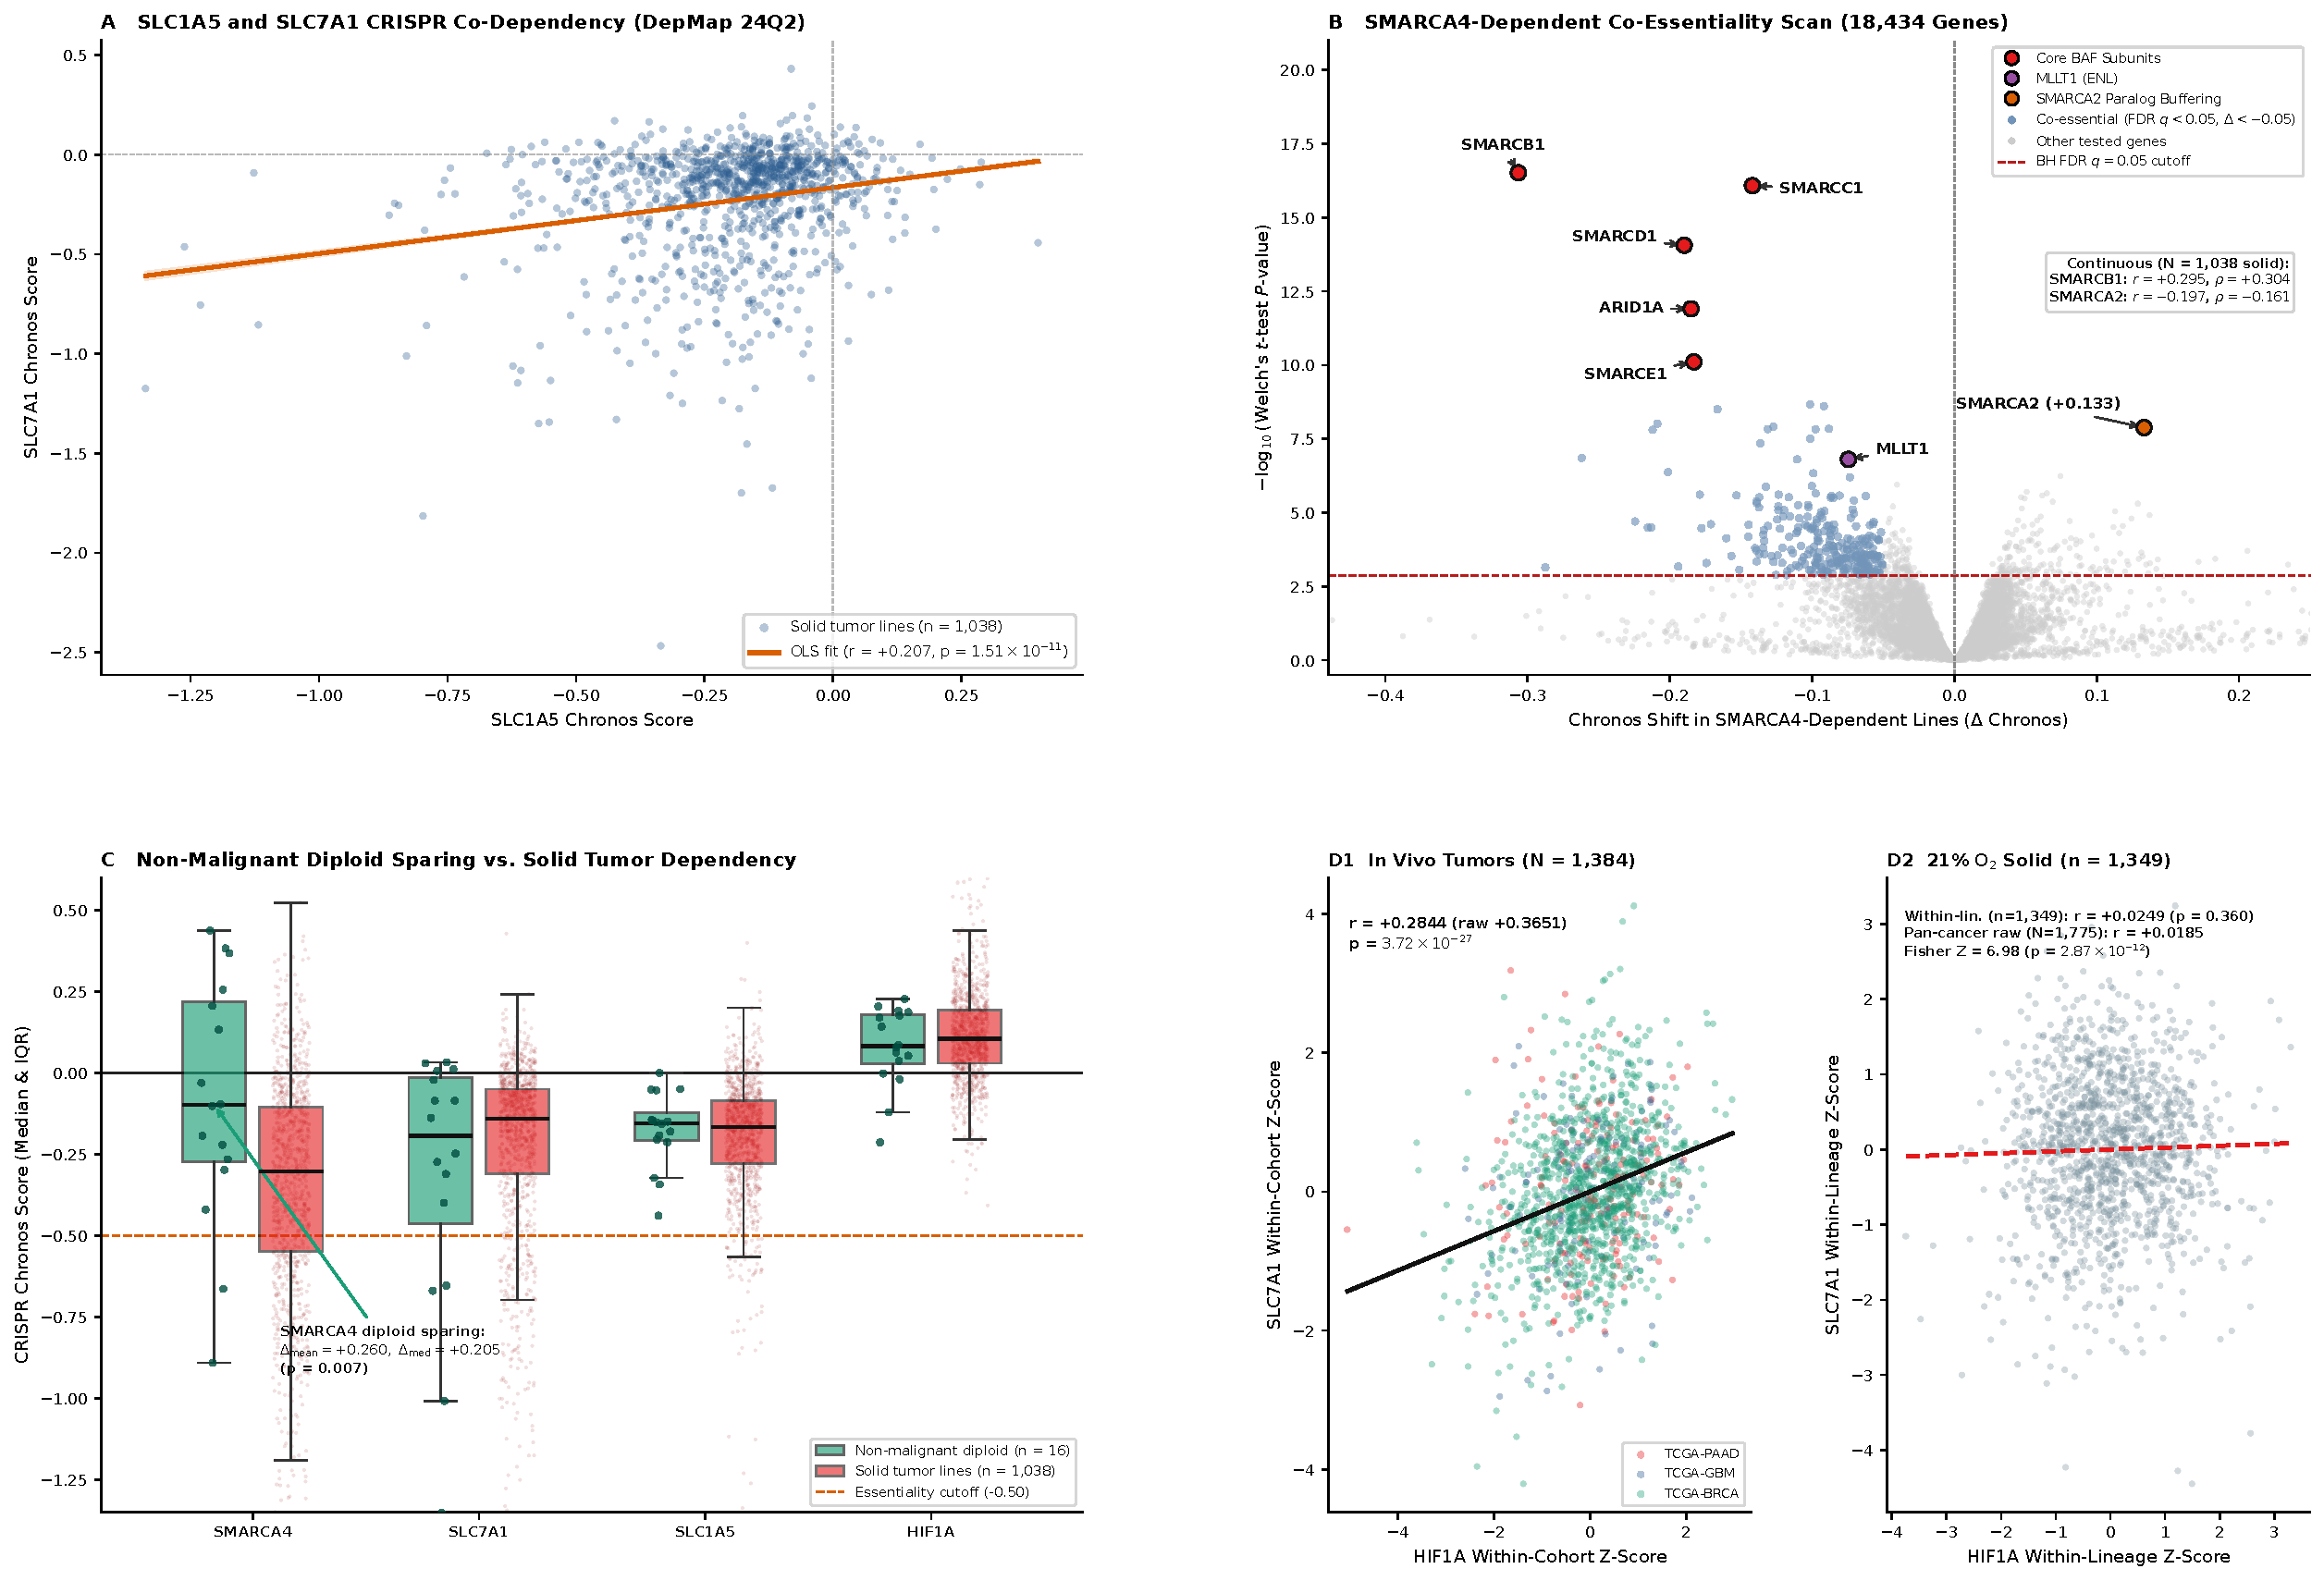
\includegraphics[width=\textwidth]{Figure_1_Final.pdf}
\caption{\textbf{Pan-Cancer Solute Carrier Co-Dependency, Core BAF Co-Essentiality, Diploid Sparing, and Normoxic $21\%\ \text{O}_2$ Uncoupling.} (A) Broad DepMap 24Q2 CRISPR Chronos co-dependency between \textit{SLC1A5} and \textit{SLC7A1} across $1,038$ solid tumor lines ($r = +0.207$, $p = 1.51 \times 10^{-11}$, BH FDR $q = 1.51 \times 10^{-10}$). (B) Genome-wide co-essentiality volcano plot ($18,434$ genes) comparing \textit{SMARCA4}-dependent ($n = 299$) versus \textit{SMARCA4}-independent ($n = 251$) solid tumor lines alongside continuous $N = 1,038$ correlations, highlighting core BAF co-essentiality, \textit{MLLT1}, and \textit{SMARCA2} paralog buffering ($\Delta = +0.133$). (C) Non-malignant diploid sparing ($n = 16$ vs.\ $1,038$ solid tumor lines; y-axis focused on [$-1.35$, $0.60$]; full \textit{SLC7A1} range shown in A), highlighting attenuated single-gene \textit{SMARCA4} dependency in diploid lines ($\Delta_{\text{mean}} = +0.260$, $\Delta_{\text{median}} = +0.205$, $p = 0.007$). (D) Within-cohort Z-scored \textit{HIF1A}--\textit{SLC7A1} coupling across $1,384$ primary TCGA tumors ($r = +0.2844$, $p = 3.72 \times 10^{-27}$; raw $r = +0.3651$) versus collapse in normoxic $21\%\ \text{O}_2$ solid DepMap cell lines ($n = 1,349$ unique lines, within-lineage $r = +0.0249$, $p = 0.360$, Fisher $Z = 6.98$, $p = 2.87 \times 10^{-12}$; pan-cancer raw $N = 1,775$, $r = +0.0185$).}
\label{fig:figure1}
\end{figure*}

\subsection{A Priori Two-Gene Score, Bulk PDAC Attenuation, and Multi-Cohort Meta-Analysis}
To test clinical relevance without fitting cohort-specific weights, we defined an unweighted a priori two-gene score from the upstream transcriptional regulators (\textit{SMARCA4} and \textit{HIF1A}) and standardized it within each cohort to mean 0 and SD 1:
\begin{equation}
\text{Risk Score} = Z\bigl(z_{\textit{SMARCA4}} + z_{\textit{HIF1A}}\bigr)
\end{equation}
We omitted downstream targets (\textit{SLC7A1}, \textit{SLC1A5}, and \textit{ABCB1}) after confirming that neither \textit{SLC7A1} (univariate $\text{HR} = 0.968$, $p = 0.752$) nor \textit{ABCB1} (univariate $\text{HR} = 0.802$, $p = 0.023$; four-gene $\beta = -0.3419$, $p = 0.009$) conferred adverse hazard in TCGA-PAAD ($N = 176$, 92 deaths). Within that complete-case four-gene model ($N = 168$, 89 deaths, adjusted for age, stage, and ABSOLUTE purity), only \textit{HIF1A} associated independently with shorter survival ($\beta = +0.3192$, $p = 0.014$; univariate $\text{HR} = 1.262$), whereas \textit{SMARCA4} ($\beta = -0.1380$, $p = 0.337$) and \textit{SLC7A1} ($\beta = -0.0351$) were null.

In bulk TCGA-PAAD, the unweighted \textit{SMARCA4} + \textit{HIF1A} score did not predict overall survival after adjusting for age, stage, and ABSOLUTE purity ($N = 168$, 89 deaths; per-SD $\text{HR} = 1.143$, $p = 0.273$, C-index $= 0.579$; Figure~2A1). Median dichotomization ($\text{HR} = 1.093$, $p = 0.679$) and age- plus stage-adjusted modeling without purity ($N = 174$, $\text{HR} = 1.081$, $p = 0.501$) were also null. Restricting TCGA-PAAD to histologically confirmed ductal PDAC from the Raphael et al.\ whitelist \cite{raphael2017} ($N = 148$, $\text{HR} = 0.950$, $p = 0.669$), cBioPortal ductal cases ($N = 138$, $\text{HR} = 0.996$), or non-PNET tumors ($N = 161$, $\text{HR} = 1.066$) did not restore signal. Similarly, adding the two-gene score to \textit{MKI67}, age, and stage left model log-likelihood unchanged ($\chi^2_{\text{LRT}}(1) = 0.00$, $p = 0.997$). Bulk TCGA-PAAD survival thus remains null across full, purity-adjusted (median ABSOLUTE purity $0.350$), and ductal-restricted models ($p = 0.273\text{--}0.974$), indicating that post-translational HIF-1$\alpha$ regulation and tumor heterogeneity limit bulk transcriptomic surrogates. In the independent ICGC/PCAWG-PAAD cohort ($N = 71$, 48 deaths; stage and purity unavailable), the score reached significance after age and sex adjustment (per-SD $\text{HR} = 1.504$, $95\%$ CI [1.109--2.041], $p = 0.009$, C-index $= 0.658$), although borderline log-rank separation ($p = 0.060$; Figure~2A2) leaves that replication tentative. Whether opposing malignant effects of \textit{SMARCA4} and hypoxia signaling or stromal composition explain the divergence against ICGC/PCAWG-PAAD requires dedicated deconvolution follow-up.

Across all 10 primary cohorts totaling $5,102$ patients ($2,162$ deaths; Figure~2B1--D), DerSimonian-Laird random-effects meta-analysis yielded a modest overall per-SD hazard ($\text{HR}^* = 1.144$, $95\%$ CI [1.089--1.203], $p = 9.10 \times 10^{-8}$, $I^2 = 16.1\%$). Single-gene decomposition revealed that \textit{SMARCA4} generated most of the signal ($\text{HR}^* = 1.153$, $p = 2.82 \times 10^{-4}$, $I^2 = 60.6\%$), while \textit{HIF1A} mRNA alone was null ($\text{HR}^* = 1.047$, $p = 0.222$, $I^2 = 60.3\%$) and reached significance only in TCGA-BLCA ($\text{HR} = 1.205$, $p = 0.017$) and purity-adjusted TCGA-PAAD ($\text{HR} = 1.319$, $p = 0.023$). Averaging \textit{SMARCA4} with null \textit{HIF1A} shrank apparent heterogeneity from $I^2 > 60\%$ to $16.1\%$ by attenuating cohort-level extremes rather than through synergistic risk. To test whether tumor proliferation confounded those hazard estimates, we adjusted every primary cohort for \textit{MKI67} using TCGA, METABRIC, and the full $24,326$-gene public CGGA-325 RSEM transcriptome. Across the eight primary TCGA cohorts ($N = 3,323$), adding \textit{MKI67} lowered the pooled hazard from $\text{HR}^* = 1.149$ to $\text{HR}^* = 1.095$ ($p = 0.023$, $I^2 = 31.6\%$). In CGGA-325 ($N = 313$, 218 deaths), \textit{MKI67} control completely abolished glioma stratification ($\text{HR} = 1.006$, $p = 0.943$), with \textit{TOP2A} adjustment giving a matching null result ($\text{HR} = 0.949$, $p = 0.505$). BRCA-METABRIC ($N = 1,466$) likewise attenuated from $\text{HR} = 1.114$ to $\text{HR} = 1.085$ ($p = 0.025$), leaving a complete 10-cohort \textit{MKI67}-adjusted estimate of $\text{HR}^* = 1.084$ ($95\%$ CI [1.026--1.146], $p = 0.004$, $I^2 = 20.3\%$). Only clear cell renal (TCGA-KIRC: $\text{HR} = 1.239$, $p = 0.007$) and urothelial bladder (TCGA-BLCA: $\text{HR} = 1.230$, $p = 0.018$) tumors kept independent risk, and both persisted after further adjusting for PanCanAtlas ABSOLUTE purity (KIRC $N = 496$: $+\text{Purity}$ $\text{HR} = 1.314$, $p = 4.74 \times 10^{-4}$; $+\textit{MKI67}+\text{Purity}$ $\text{HR} = 1.282$, $p = 0.002$; BLCA $N = 393$: $+\text{Purity}$ $\text{HR} = 1.195$, $p = 0.035$; $+\textit{MKI67}+\text{Purity}$ $\text{HR} = 1.214$, $p = 0.028$).

To verify whether this limited lineage pattern reflected cohort selection, we tested the remaining 11 adult solid TCGA cohorts that have complete survival, stage or grade, and RNA-seq profiles ($N = 4,552$, $1,241$ deaths: \texttt{LUAD}, \texttt{LUSC}, \texttt{COADREAD}, \texttt{HNSC}, \texttt{STAD}, \texttt{OV}, \texttt{UCEC}, \texttt{CESC}, \texttt{ESCA}, \texttt{THCA}, and \texttt{PRAD}). None of those 11 cohorts reached significance ($p = 0.061\text{--}0.977$; pooled $\text{HR}^* = 0.962$, $p = 0.186$). Expanding across all 19 solid TCGA cohorts ($N = 7,875$, $2,362$ deaths; Figure~2D) gave a null overall estimate ($\text{HR}^* = 1.048$, $p = 0.130$, $I^2 = 50.5\%$), which fell to $\text{HR}^* = 1.020$ ($p = 0.488$) with \textit{MKI67} control (18 stage/grade cohorts excluding \texttt{PRAD}: $\text{HR}^* = 1.044$, $p = 0.161$). Because \textit{HIF1A} mRNA poorly reflects HIF-1$\alpha$ protein stabilization, we benchmarked the 14-gene non-cell-cycle \textit{Buffa-14} hypoxia signature excluding \textit{CDKN3} \cite{buffa2010} across the same 19 cohorts ($N = 7,875$; Table~1, Figure~2D). \textit{Buffa-14} predicted shorter survival across both the eight primary TCGA cohorts ($\text{HR}^* = 1.158$, $p = 2.52 \times 10^{-6}$) and the 11 remaining TCGA cohorts ($\text{HR}^* = 1.109$, $p = 0.017$), pooling to $\text{HR}^* = 1.133$ ($95\%$ CI [1.076--1.193], $p = 2.17 \times 10^{-6}$, $I^2 = 30.7\%$) across all 19 cohorts. Adding \textit{MKI67} left \textit{Buffa-14} intact ($\text{HR}^* = 1.116$, $95\%$ CI [1.069--1.165], $p = 5.54 \times 10^{-7}$, $I^2 = 0.0\%$). In nested likelihood-ratio tests across all 19 cohorts, adding \textit{Buffa-14} to \textit{SMARCA4} + \textit{HIF1A} improved model fit both at baseline ($\chi^2_{\text{LRT}}(19) = 56.56$, $p = 1.33 \times 10^{-5}$; $N$-weighted joint $\Delta\text{C-index} = +0.0104$ over baseline $0.6878$; \textit{Buffa-14} alone $\Delta\text{C} = +0.0025$) and after \textit{MKI67} adjustment ($\chi^2_{\text{LRT}}(19) = 43.03$, $p = 1.29 \times 10^{-3}$; joint $\Delta\text{C} = +0.0070$). Conversely, adding \textit{SMARCA4} + \textit{HIF1A} onto \textit{Buffa-14} + \textit{MKI67} added no incremental fit ($\chi^2_{\text{LRT}}(19) = 29.34$, $p = 0.061$). Combining \textit{SMARCA4} with \textit{Buffa-14} improved pooling across the eight primary cohorts ($\text{HR}^* = 1.220$, $p = 3.05 \times 10^{-10}$; $+\textit{MKI67}$ $\text{HR}^* = 1.167$), but remained null across the 11 remaining cohorts ($\text{HR}^* = 1.008$, $p = 0.813$). Systemic hypoxia programs thus drive broad solid-tumor risk, whereas bulk \textit{HIF1A} mRNA is an insensitive hypoxic readout and \textit{SMARCA4} hazard stays lineage-confined.

Finally, because breast cancer accounts for $48.6\%$ of the unified 11-cohort pool ($2,516/5,173$ patients; $\text{HR}^* = 1.155$, $p = 1.96 \times 10^{-7}$, $I^2 = 27.7\%$), we audited breast confounding and proportional hazards assumptions explicitly. Non-breast primary cohorts retained pooled significance without breast tumors ($\text{HR}^* = 1.152$, $p = 7.27 \times 10^{-5}$, $I^2 = 28.9\%$, $N = 2,586$; nine non-breast cohorts including ICGC/PCAWG-PAAD: $\text{HR}^* = 1.166$, $N = 2,657$). In BRCA-METABRIC, omitting 513 stage-missing cases caused no selection bias: age-adjusted models across all $1,979$ complete-OS tumors ($\text{HR} = 1.111$, $p = 3.91 \times 10^{-4}$) matched the $1,466$ stage-complete subset ($\text{HR} = 1.115$, $p = 0.002$). However, adjusting for PAM50 subtype abolished risk in TCGA-BRCA ($N = 950$, $\text{HR} = 1.052$, $p = 0.611$) and attenuated BRCA-METABRIC under PAM50/Claudin-low ($\text{HR} = 1.070$, $p = 0.068$), ER/PR/HER2 status ($\text{HR} = 1.050$, $p = 0.192$), or both ($\text{HR} = 1.035$, $p = 0.361$), showing that breast stratification tracks ER-negative and basal-like subtypes. Across Schoenfeld residual tests in all 22 cohorts, 19 satisfied proportional hazards ($p = 0.112\text{--}0.979$), including ICGC/PCAWG-PAAD ($p = 0.353$) and all 11 expanded TCGA cohorts; non-proportionality occurred only in null TCGA-GBM ($p = 0.017$), TCGA-BRCA ($p = 0.046$), and 25-year METABRIC ($p = 0.0001$), where hazard concentrated in the first 5~years ($\text{HR} = 1.306$, $p = 7.61 \times 10^{-7}$) and 10~years ($\text{HR} = 1.172$) before late competing mortality.

\begin{table*}[t]
\centering
\caption{\textbf{Unified Multi-Cohort Multivariable Cox Proportional Hazards Summary and 19-Cohort \textit{Buffa-14} Hypoxia Benchmark.} Meta-analytic estimates use DerSimonian-Laird random-effects pooling on continuous per-SD Z-scores ($Z(z_{\textit{SMARCA4}} + z_{\textit{HIF1A}})$ unless labeled \textit{Buffa-14}). TCGA-PAAD adjusts for Age, Stage, and PanCanAtlas/Raphael ABSOLUTE Purity ($N = 168$ of 176 primary cases); ICGC/PCAWG-PAAD ($N = 71$) adjusts for Age and Sex (stage and purity unavailable).}
\scriptsize
\setlength{\tabcolsep}{4pt}
\resizebox{\textwidth}{!}{%
\begin{tabular}{@{}lccccccc>{\raggedright\arraybackslash}p{3.9cm}@{}}
\toprule
\textbf{Cohort} & \textbf{$N$} & \textbf{Deaths} & \textbf{Per-SD HR [95\% CI]} & \textbf{Wald $p$} & \textbf{Median HR [95\% CI]} & \textbf{Median $p$} & \textbf{C-Idx} & \textbf{Covariates / Notes} \\
\midrule
TCGA-PAAD & 168 & 89 & 1.143 [0.900--1.452] & 0.273 & 1.093 [0.717--1.666] & 0.679 & 0.579 & Age, Stage, ABSOLUTE Purity \\
CGGA-325 (Diffuse Glioma II--IV) & 313 & 218 & 1.193 [1.050--1.355] & 0.007 & 1.684 [1.264--2.245] & $3.73 \times 10^{-4}$ & 0.717 & Age, Grade, IDH, MGMT \\
TCGA-KIRC (Clear Cell Renal) & 531 & 175 & 1.289 [1.114--1.492] & $6.61 \times 10^{-4}$ & 1.647 [1.212--2.238] & 0.001 & 0.764 & Age, Stage \\
TCGA-SARC (Soft-Tissue Sarcoma) & 253 & 96 & 1.183 [0.963--1.453] & 0.110 & 1.491 [0.992--2.240] & 0.055 & 0.584 & Age \\
TCGA-SKCM (Cutaneous Melanoma) & 417 & 196 & 1.108 [0.956--1.283] & 0.172 & 1.272 [0.952--1.698] & 0.103 & 0.648 & Age, Stage \\
TCGA-BRCA (Breast Carcinoma) & 1,050 & 143 & 1.187 [1.012--1.393] & 0.035 & 1.385 [0.994--1.930] & 0.054 & 0.762 & Age, Stage \\
TCGA-LIHC (Hepatocellular) & 343 & 118 & 1.172 [0.977--1.407] & 0.088 & 1.213 [0.838--1.755] & 0.306 & 0.643 & Age, Stage \\
TCGA-BLCA (Urothelial Bladder) & 403 & 177 & 1.206 [1.024--1.419] & 0.024 & 1.530 [1.132--2.068] & 0.006 & 0.668 & Age, Stage \\
BRCA-METABRIC (Breast OS) & 1,466 & 823 & 1.114 [1.040--1.192] & 0.002 & 1.238 [1.078--1.421] & 0.002 & 0.641 & Age, Stage \\
TCGA-GBM (WHO Grade IV) & 158 & 127 & 0.922 [0.778--1.093] & 0.348 & 0.802 [0.565--1.140] & 0.219 & 0.618 & Age \\
\midrule
TCGA-PAAD (Pure Ductal PDAC) & 148 & 82 & 0.950 [0.750--1.202] & 0.669 & 0.780 [0.504--1.209] & 0.267 & 0.578 & Age, Stage, ABSOLUTE Purity \\
ICGC/PCAWG-PAAD & 71 & 48 & 1.504 [1.109--2.041] & 0.009 & 1.821 [1.017--3.263] & 0.044 & 0.658 & Age, Sex (stage unavailable) \\
\midrule
8-Cohort Non-Breast Primary Meta ($I^2 = 28.9\%$) & 2,586 & 1,196 & 1.152 [1.074--1.235] & $7.27 \times 10^{-5}$ & -- & -- & -- & Excl.\ TCGA-BRCA, METABRIC \& ICGC-PAAD \\
9-Cohort Non-Breast Meta ($I^2 = 36.7\%$) & 2,657 & 1,244 & 1.166 [1.083--1.255] & $4.22 \times 10^{-5}$ & -- & -- & -- & Excl.\ TCGA-BRCA \& METABRIC \\
10-Cohort Primary Meta ($I^2 = 16.1\%$) & 5,102 & 2,162 & 1.144 [1.089--1.203] & $9.10 \times 10^{-8}$ & -- & -- & -- & 10 Primary Cohorts \\
11-Cohort Unified Meta ($I^2 = 27.7\%$) & 5,173 & 2,210 & 1.155 [1.094--1.220] & $1.96 \times 10^{-7}$ & -- & -- & -- & 10 Primary + ICGC/PCAWG-PAAD \\
19-Cohort Expanded Solid TCGA ($I^2 = 50.5\%$) & 7,875 & 2,362 & 1.048 [0.986--1.114] & 0.130 & -- & -- & 0.688 & 8 Primary + 11 Additional TCGA \\
19-Cohort Solid TCGA: \textit{Buffa-14} ($I^2 = 30.7\%$) & 7,875 & 2,362 & 1.133 [1.076--1.193] & $2.17 \times 10^{-6}$ & -- & -- & 0.690 & \textit{Buffa-14} vs.\ 2-gene LRT $\chi^2(19)=56.56$, $p=1.33\times 10^{-5}$ \\
19-Cohort Solid TCGA: \textit{Buffa-14} (+\textit{MKI67}, $I^2 = 0.0\%$) & 7,875 & 2,362 & 1.116 [1.069--1.165] & $5.54 \times 10^{-7}$ & -- & -- & 0.696 & \textit{Buffa-14} + \textit{MKI67} LRT $\chi^2(19)=43.03$, $p=1.29\times 10^{-3}$ \\
\bottomrule
\end{tabular}%
}
\end{table*}

\begin{figure*}[!t]
\centering
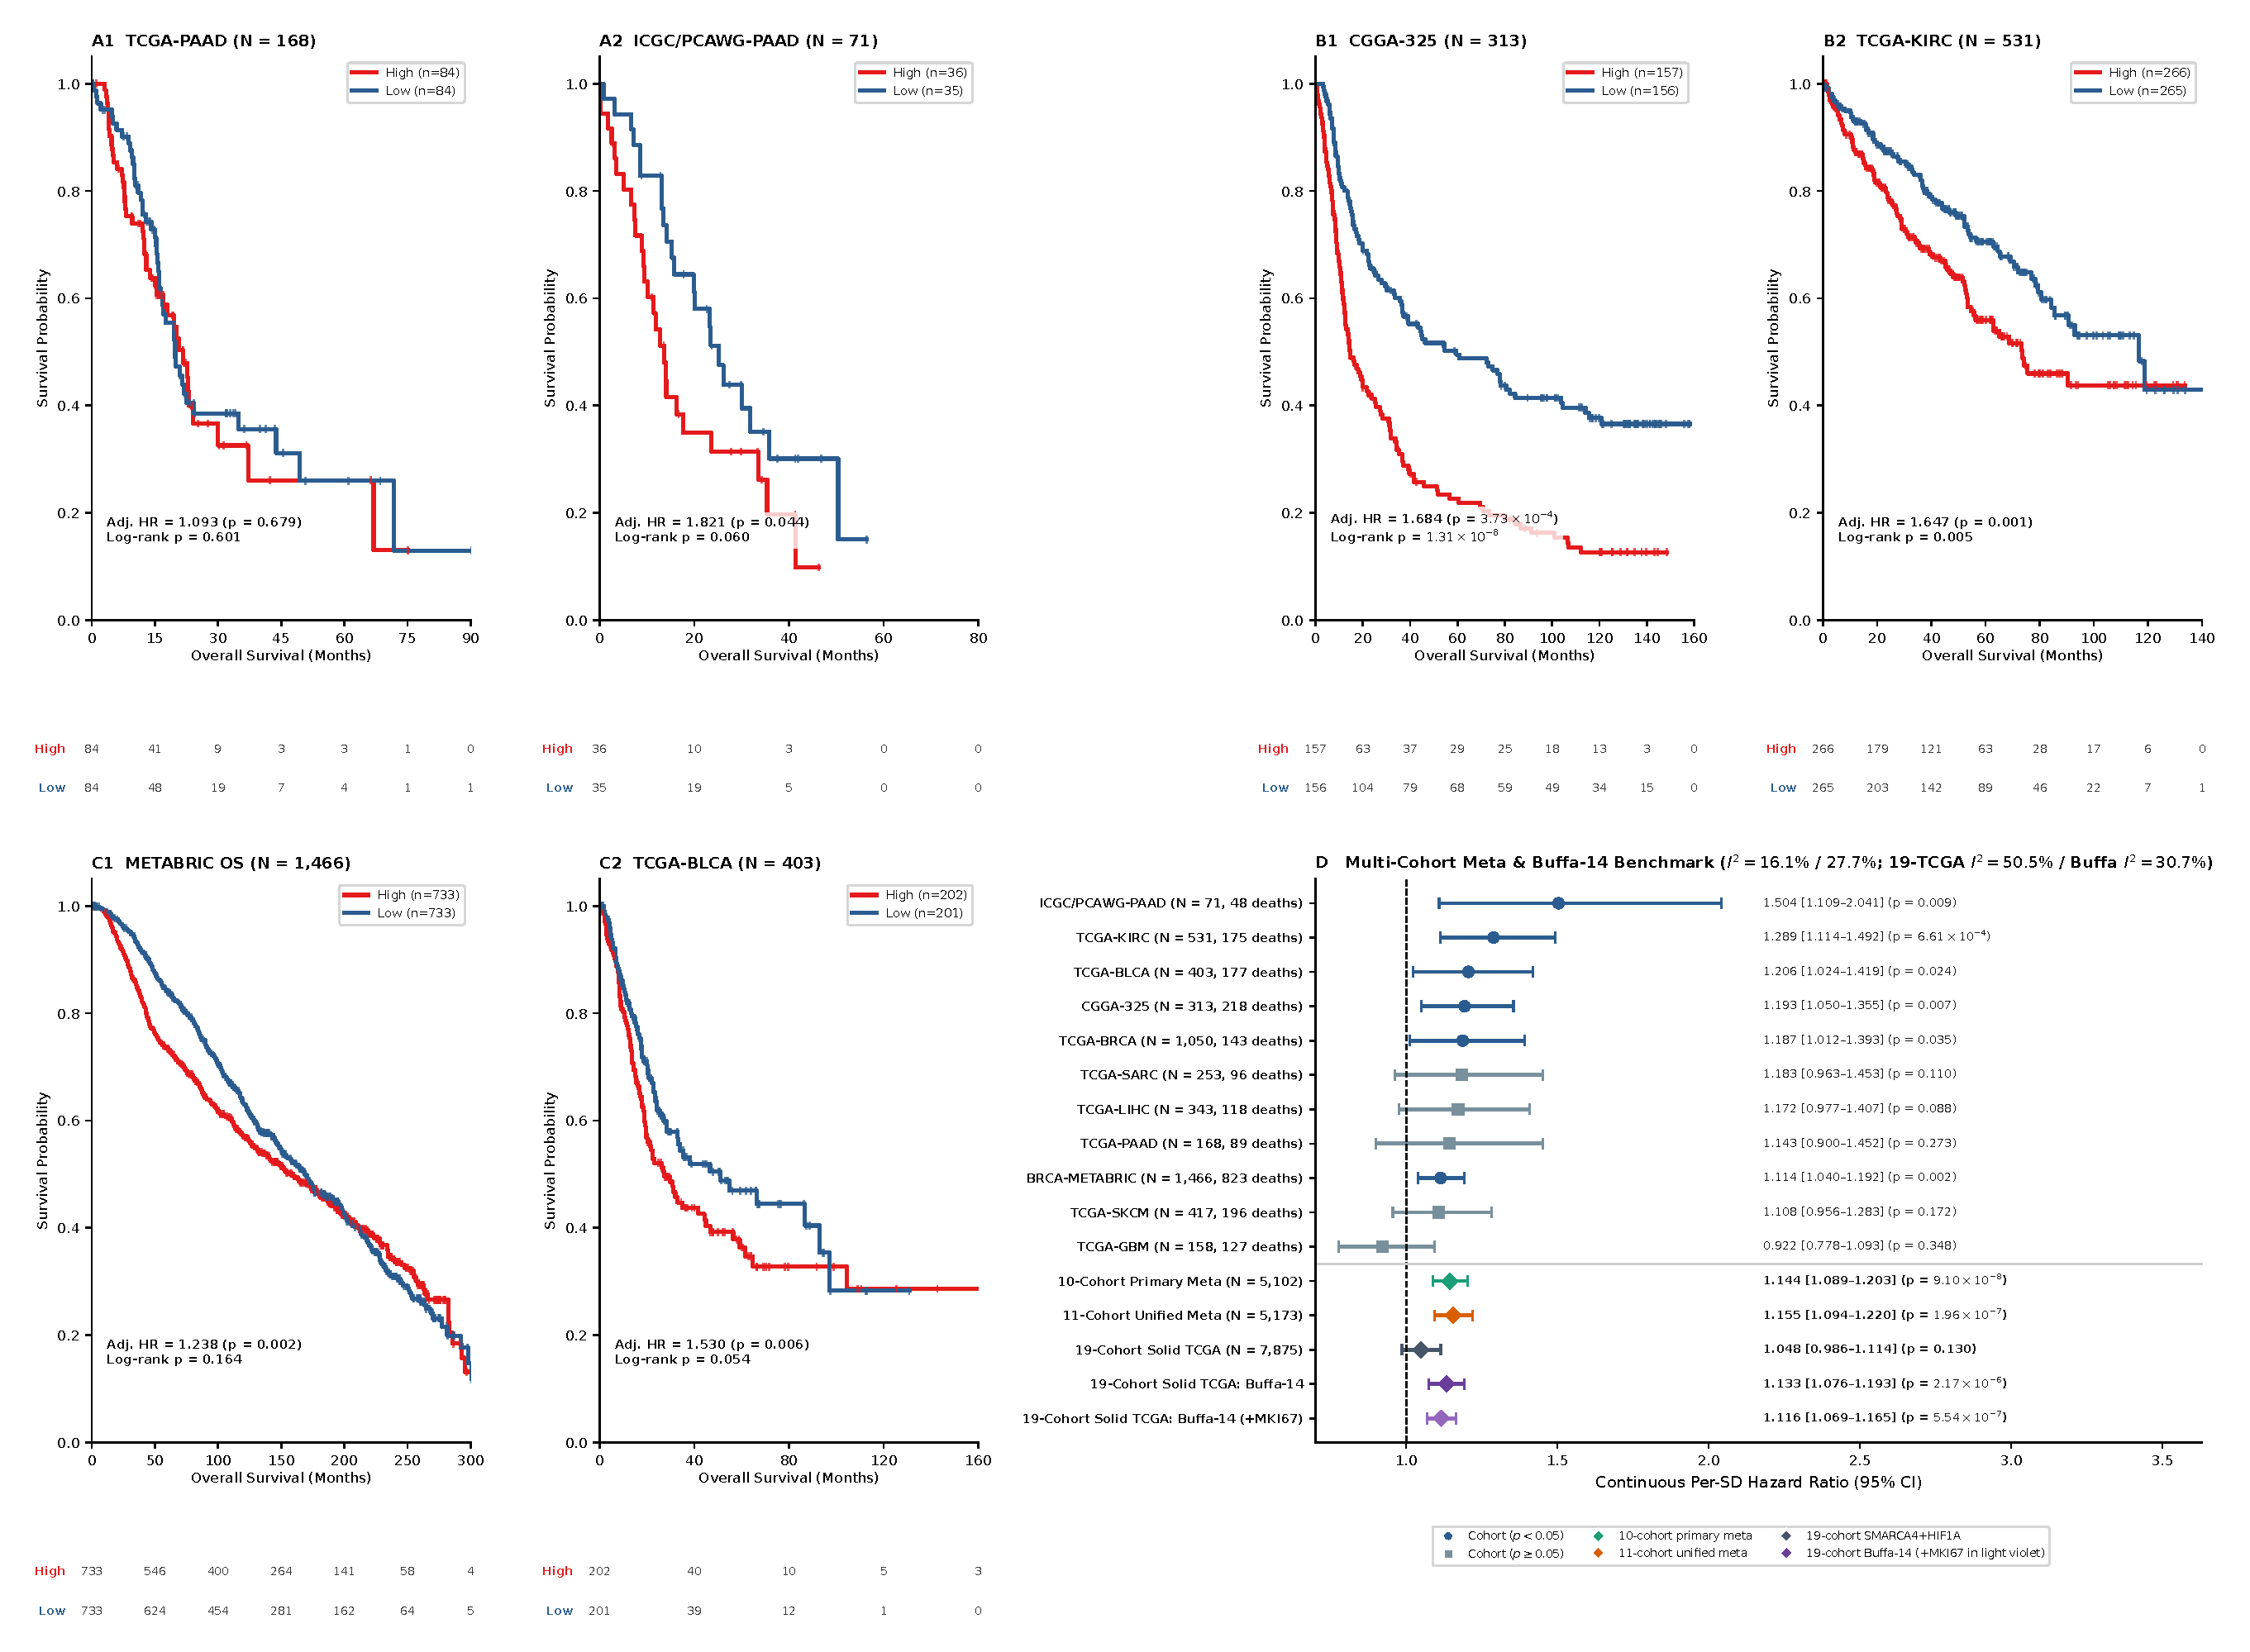
\includegraphics[width=\textwidth]{Figure_2_Final.pdf}
\caption{\textbf{Uniform Median-Split Kaplan-Meier Stratification and Unified Multi-Cohort Meta-Analysis.} (A1--A2) Pancreatic overall survival curves for the unweighted $Z(z_{\textit{SMARCA4}} + z_{\textit{HIF1A}})$ score comparing complete-case TCGA-PAAD ($N = 168$) and age/sex-adjusted ICGC/PCAWG-PAAD ($N = 71$). (B1--B2, C1--C2) Median-split Kaplan-Meier curves in CGGA-325 ($N = 313$), TCGA-KIRC ($N = 531$), METABRIC ($N = 1,466$), and TCGA-BLCA ($N = 403$) with censoring ticks, number-at-risk tables, adjusted HRs, and log-rank $p$-values. (D) Continuous per-SD hazard ratio forest plot showing all 11 individual cohorts alongside the 10-cohort primary meta-analysis ($\text{HR}^* = 1.144$, $I^2 = 16.1\%$), the unified 11-cohort synthesis ($\text{HR}^* = 1.155$, $I^2 = 27.7\%$), the expanded 19-cohort solid TCGA pool ($\text{HR}^* = 1.048$, $p = 0.130$, $I^2 = 50.5\%$, $N = 7,875$), and the 19-cohort \textit{Buffa-14} benchmark ($\text{HR}^* = 1.133$, $I^2 = 30.7\%$; +\textit{MKI67} $\text{HR}^* = 1.116$, $I^2 = 0.0\%$).}
\label{fig:figure2}
\end{figure*}

\subsection{Lineage-Controlled Pharmacogenomics, Combination Synergy, and Biomarker Gates}
We next asked whether baseline \textit{SMARCA4} + \textit{HIF1A} expression predicts therapeutic sensitivity across $m = 286$ drugs in Sanger GDSC2 under ambient $21\%\ \text{O}_2$ culture (Figure~3A). Using lineage-controlled Type~II ANOVA on empirical $1 - \text{AUC}$ avoided $\text{IC}_{50}$ curve extrapolations above the $10\ \mu\text{M}$ screening ceiling. Overall effect sizes were modest across the screen (median partial $R^2$, $\eta_p^2 = 0.176\%$; screen-wide maximum $3.53\%$), with 35 nominal associations ($p < 0.05$, 29 sensitizing). Only one compound cleared a strict 5\% Benjamini-Hochberg FDR cutoff---the BCL2/BCL-XL inhibitor Navitoclax ($F(1, 570) = 14.32$, $\eta_p^2 = 2.45\%$, $p = 1.71 \times 10^{-4}$, $q = 0.049$)---while nine of $286$ compounds cleared 10\% FDR ($\eta_p^2 = 1.55\%\text{--}2.63\%$). Alongside Navitoclax, seven additional FDR $< 10\%$ hits showed weak sensitization: ABT737 ($F = 11.38$, $q = 0.059$), WEHI-539 ($F = 10.90$, $q = 0.059$), Cisplatin ($F = 12.80$, $q = 0.055$), Oxaliplatin ($F = 8.96$, $q = 0.091$), Elephantin ($F = 11.25$, $q = 0.059$), Entinostat ($F = 9.84$, $q = 0.086$), and Uprosertib ($F = 9.23$, $q = 0.091$). The ninth hit, PRMT5 inhibitor GSK591, tracked mild resistance ($\beta = -0.0046$, $F = 9.17$, $q = 0.091$). In secondary $\ln(\text{IC}_{50})$ testing, top hits pointed in the same direction, though zero compounds cleared 10\% FDR (minimum $q = 0.110$). Topoisomerase~I and PARP1/2 inhibitors showed weaker nominal $1 - \text{AUC}$ trends---Irinotecan ($q = 0.126$), Niraparib ($q = 0.234$), Rucaparib ($q = 0.242$), Camptothecin ($q = 0.292$), Olaparib ($q = 0.354$), and Talazoparib ($q = 0.354$)---while taxanes, 5-Fluorouracil, SN-38 ($p = 0.980$), AZD5153 ($p = 0.512$), and AZD5991 ($p = 0.335$) were null.

To distinguish direct pathway sensitization from rapid cell division, we added \textit{MKI67} mRNA alongside tissue lineage in the GDSC2 ANOVA models. Every one of the nine FDR $< 10\%$ drugs kept nominal significance ($p = 6.43 \times 10^{-4}$ to $0.011$), led by WEHI-539 ($F = 10.90 \rightarrow 11.78$), Navitoclax ($14.32 \rightarrow 10.94$), Cisplatin ($12.80 \rightarrow 9.94$), ABT737 ($11.38 \rightarrow 9.67$), and Uprosertib ($9.23 \rightarrow 8.32$). By contrast, \textit{MKI67} adjustment weakened PARP1/2 and TOP1 signals below significance for Niraparib ($p = 0.072$), Camptothecin ($p = 0.103$), Olaparib ($p = 0.120$), and Talazoparib ($p = 0.136$), leaving only attenuated Irinotecan activity ($F = 7.88 \rightarrow 4.52$, $p = 0.034$). Proliferation rates therefore account for much of the apparent normoxic TOP1 and PARP1/2 relationship.

We next examined whether combination regimens overcome normoxic monotherapy uncoupling across $84,055$ Sanger GDSC matrix rows ($69,121$ solid rows) spanning five screens (\texttt{gdsc-007}--\texttt{gdsc-010} and \texttt{sandpiper-01}) \cite{jaaks2022,bashi2024} (Figure~3B1--B2). Because choosing the peak $3 \times 3$ Bliss window across sliding $7 \times 7$ grids introduces positive selection bias, we compared each pair against the median across all $k = 109$ canonical pairs tested in at least 30 solid lines ($+0.0662$). Olaparib plus SN-38 ($479$ lines; median $+0.1543$, $\Delta = +0.0881$, Wilcoxon $p = 9.19 \times 10^{-67}$, 89.9th percentile) and Capivasertib plus Selumetinib ($586$ lines; median $+0.0872$, $p = 4.18 \times 10^{-24}$, 62.4th percentile) exceeded empirical background. BRD4 + MCL1 co-inhibition with AZD5153 plus AZD5991 sat near background overall ($587$ lines; median $+0.0626$, 45.0th percentile), though $199$ lines peaked at the lowest \texttt{(D1, D1)} anchor (mean peak Bliss $+0.156$). After adjusting for tissue lineage, however, zero of three combinations tracked baseline \textit{SMARCA4} + \textit{HIF1A} expression: AZD5153 plus AZD5991 ($F(1, 450) = 2.45$, $p = 0.118$), Olaparib plus SN-38 ($F(1, 345) = 3.35$, $p = 0.068$), and Capivasertib plus Selumetinib ($F(1, 449) = 0.26$, $p = 0.613$) were all uncoupled.

By contrast, known single-gene response gates held strongly on empirical $1 - \text{AUC}$ across solid lines (Figure~3C--D). Higher \textit{SLFN11} expression tracked greater activity for SN-38 ($n = 588$, lineage-adjusted $r_{\text{adj}} = +0.1775$, $p = 2.19 \times 10^{-5}$) and Olaparib ($n = 595$, $r_{\text{adj}} = +0.2486$, $p = 1.66 \times 10^{-9}$), separating silenced lines ($< 1.0\ \log_2(\text{TPM}+1)$) for SN-38 ($\Delta(1 - \text{AUC}) = +0.0592$, Mann-Whitney $p = 8.35 \times 10^{-9}$) and Olaparib ($\Delta = +0.0089$, $p = 3.16 \times 10^{-5}$) in concordance with $\ln(\text{IC}_{50})$ ($r_{\text{adj}} = -0.3883$ and $-0.2077$). Similarly, the mitochondrial pore protein \textit{BAK1} tracked AZD5991 $1 - \text{AUC}$ ($n = 462$, $r_{\text{adj}} = +0.1553$, $p = 0.001$; median-split $\Delta = +0.0316$, $p = 0.009$; $\ln(\text{IC}_{50})$ $r_{\text{adj}} = -0.1835$), while \textit{BAX} showed no relationship ($r_{\text{adj}} = -0.0516$, $p = 0.280$). Both gates extended to combination Bliss excess for Olaparib plus SN-38 (\textit{SLFN11} $r = +0.2934$, $p = 9.29 \times 10^{-9}$) and AZD5153 plus AZD5991 (\textit{BAK1} $r = +0.1168$, $p = 0.011$).

To evaluate normal-tissue toxicity risk without cross-pipeline batch bias, we compared TCGA primary solid tumors ($n = 9,138$) with GTEx v6 healthy tissues in the harmonized UCSC Xena Toil recompute \cite{vivian2017} (Figure~3E). Solid-tumor \textit{MCL1} expression ($114.25$ TPM, IQR $77.24\text{--}163.60$) sat modestly above Heart Left Ventricle ($44.08$ TPM, $n = 202$, $2.59\times$), Heart Atrial Appendage ($59.22$ TPM, $n = 175$, $1.93\times$), and Liver ($67.54$ TPM, $n = 110$, $1.69\times$), and actually fell below GTEx v6 Whole Blood ($135.67$ TPM, $n = 337$, $p = 8.38 \times 10^{-4}$) even with globin mRNA dilution. Normal organs also maintained substantial \textit{BRD4} ($11.92\text{--}15.57$ TPM vs.\ $22.63$ TPM in tumors; $1.45\times\text{--}1.90\times$) and \textit{BAK1} ($4.00\text{--}8.84$ TPM vs.\ $19.05$ TPM), leaving only \textit{SMARCA4} clearly enriched in tumors ($73.08$ TPM vs.\ $6.90\text{--}19.67$ TPM; $3.72\times\text{--}10.59\times$). Finally, inspecting combination \texttt{D1} anchors against monotherapy dose-response floors highlights why extrapolated $\text{IC}_{50}$ ratios must be treated carefully (Figure~3F). Across GDSC2 solid lines, median empirical $1 - \text{AUC}$ stayed near zero for AZD5991 ($0.0309$, $n = 580$) and Olaparib ($0.0407$, $n = 794$) compared with SN-38 ($0.1058$, $n = 786$) and AZD5153 ($0.1622$, $n = 582$). As a result, fitted combination-screen $\text{IC}_{50}$ medians for AZD5991 ($17,122.0\text{ nM}$, $n = 595$) and Olaparib ($141,158\text{ nM}$, $n = 604$)---like GDSC2 medians ($158,038\text{ nM}$ and $95,797\text{ nM}$)---sit well above the $10\ \mu\text{M}$ assay ceiling. Although the $1.0\text{ nM}$ AZD5153 \texttt{D1} concentration falls 245- to 272-fold below the Phase~I $30\text{ mg}$ QD total plasma $C_{\max}$ \cite{hamilton2023} ($245.4\text{ nmol/L}$ single-dose; $272.4\text{ nmol/L}$ multiple-dose), public sources lack numerical human AZD5991 $C_{\max}$ values \cite{desai2024}, human plasma unbound fractions ($f_u$) for either drug, and raw $7 \times 7$ well curves, precluding verified unbound $C_{\max, u}$ or Chou-Talalay DRI calculations.

\begin{figure*}[!t]
\centering
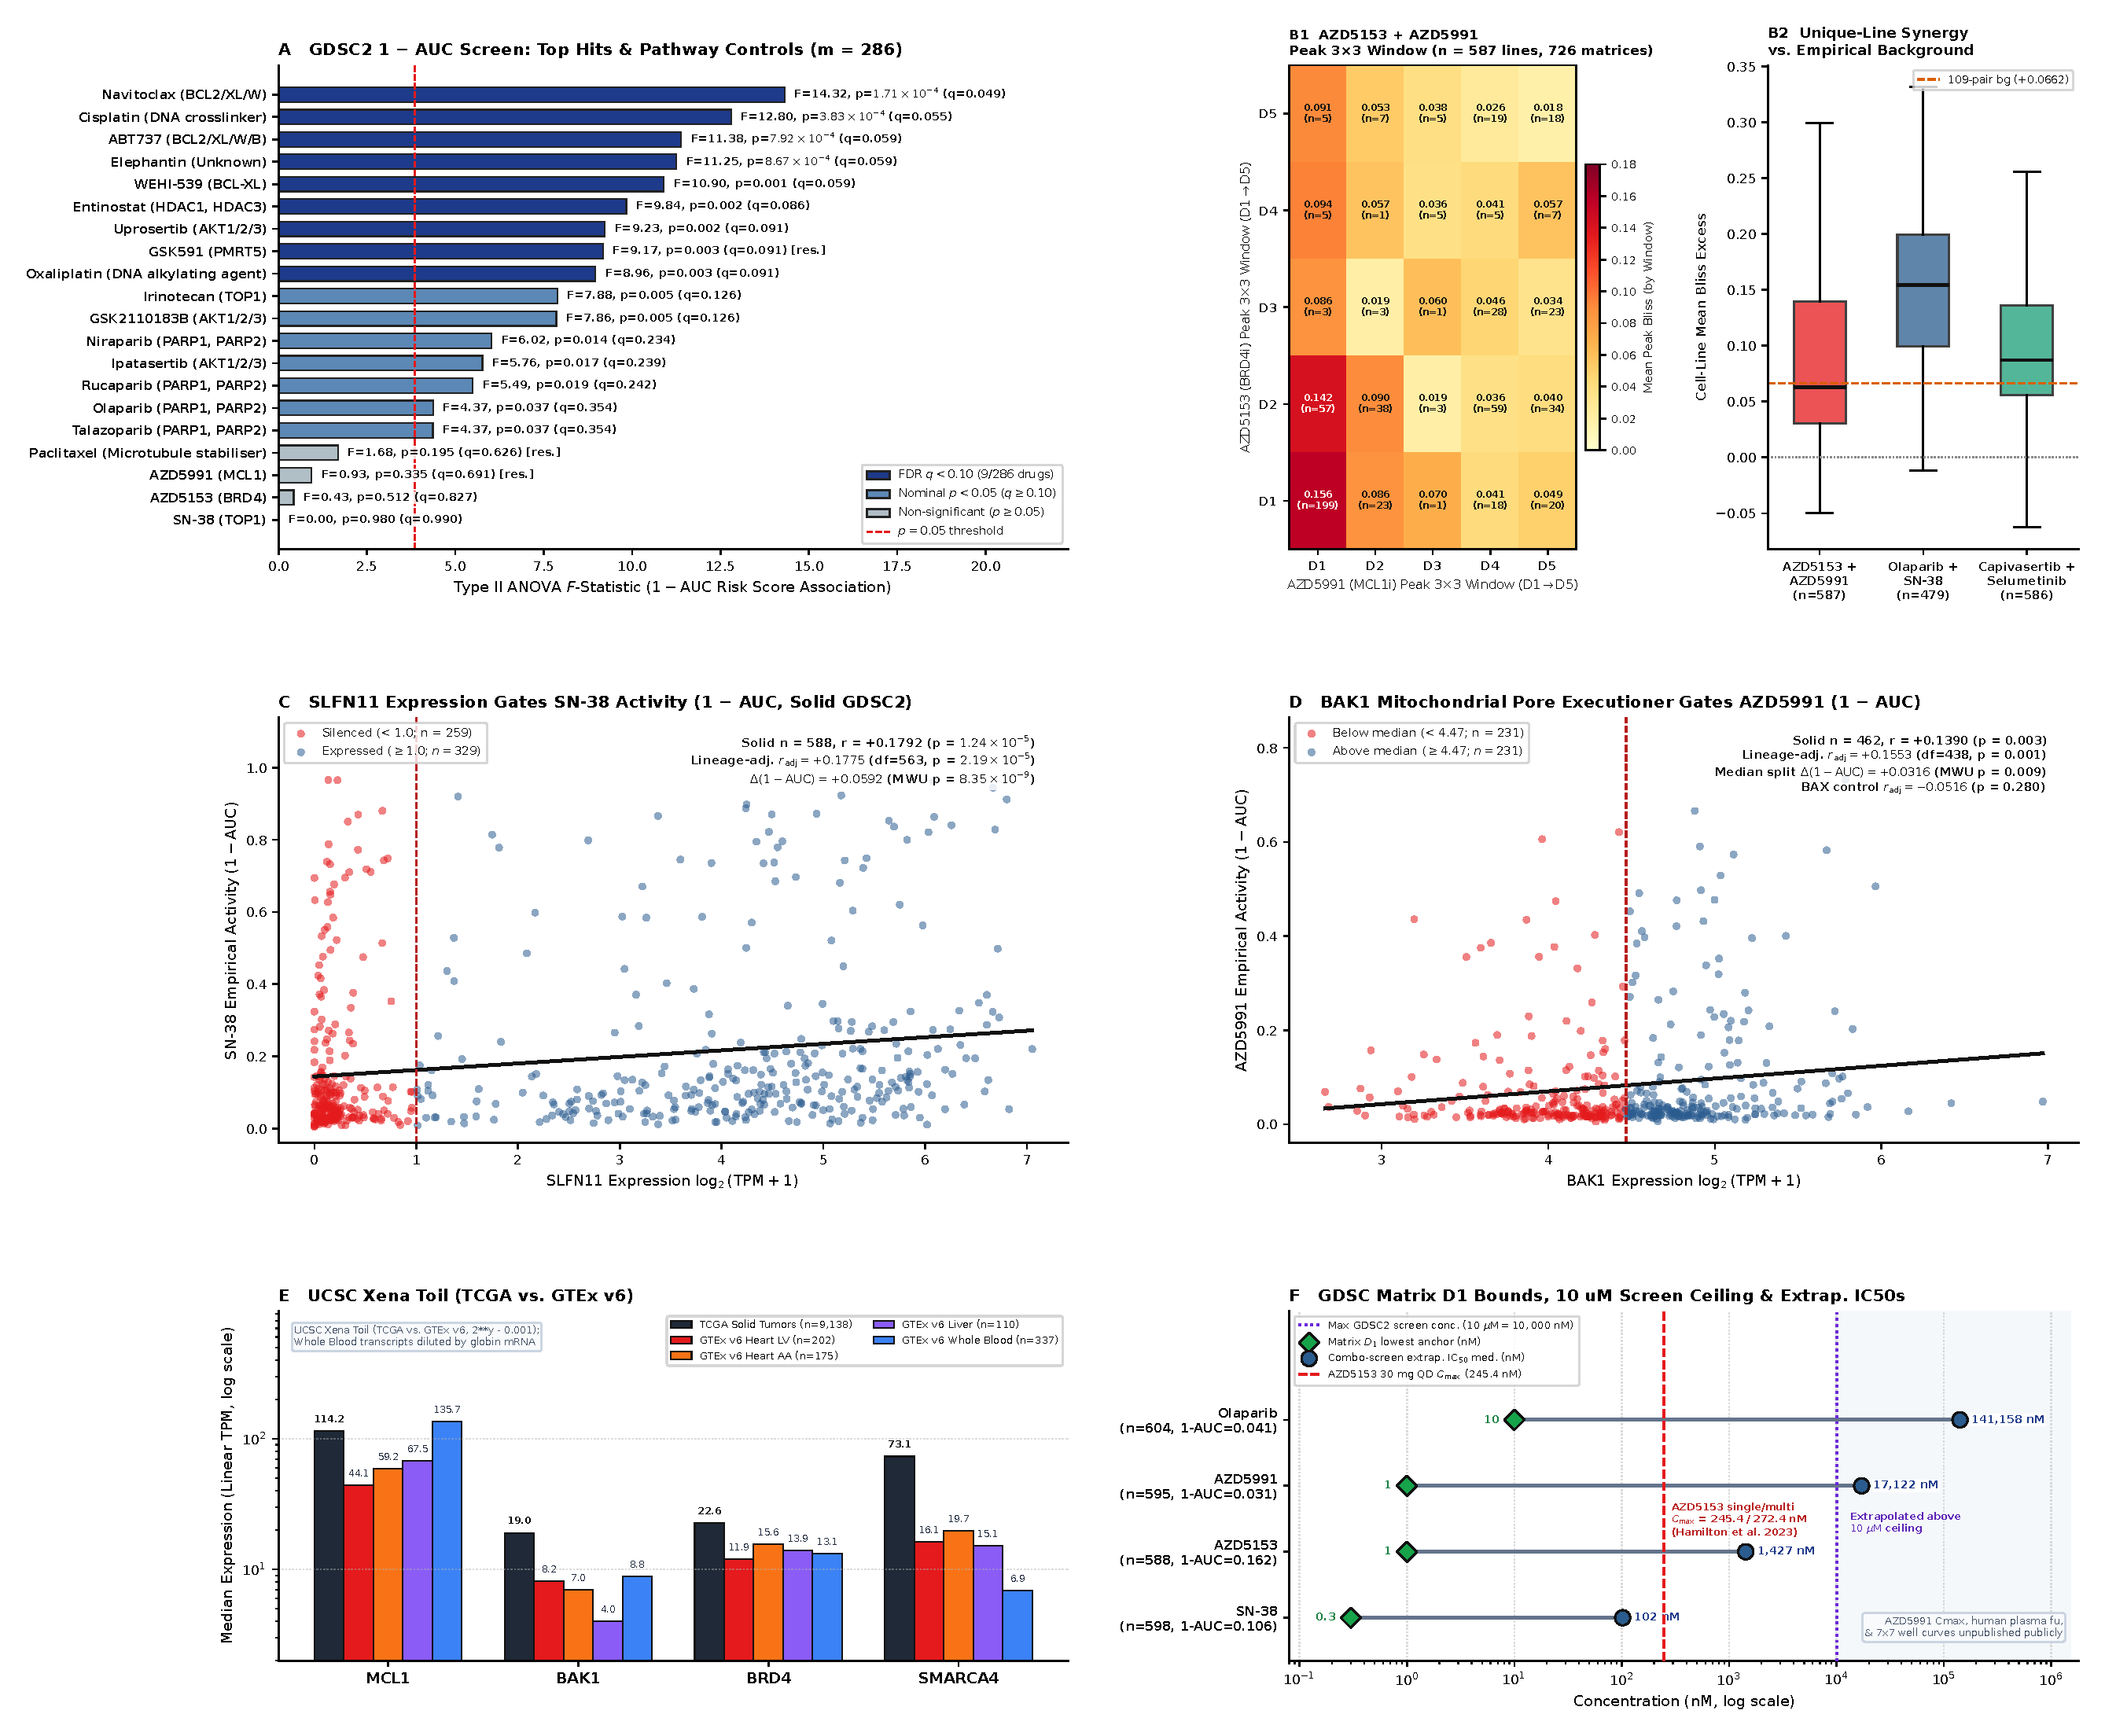
\includegraphics[width=\textwidth]{Figure_3_Final.pdf}
\caption{\textbf{Lineage-Controlled GDSC2 $1 - \text{AUC}$ Screening, Combination Bliss Synergy, Biomarker Gates, and Harmonized Toil/Exposure Counter-Screens.} (A) Type~II ANOVA $F$-statistics on empirical $1 - \text{AUC}$ across $m = 286$ GDSC2 compounds adjusted for 19--24 lineages under ambient $21\%\ \text{O}_2$ culture (20 representative compounds; $1/286$ clears FDR $q < 0.05$ and $9/286$ clear FDR $q < 0.10$, \texttt{[res.]} marks $\beta < 0$). (B1--B2) Unique-line AZD5153 plus AZD5991 mean peak $3 \times 3$ Bliss excess across $7 \times 7$ dose matrices (\texttt{D1}--\texttt{D5} start indices; modal peak $+0.156$ at \texttt{(D1, D1)}, $n = 199$) and Bliss distributions relative to the 109-pair background median ($+0.0662$, dashed orange line). (C) Axis-independent \textit{SLFN11} gate for SN-38 empirical $1 - \text{AUC}$ ($n = 588$, $r_{\text{adj}} = +0.1775$, $p = 2.19 \times 10^{-5}$). (D) Axis-independent \textit{BAK1} gate for AZD5991 empirical $1 - \text{AUC}$ ($n = 462$, $r_{\text{adj}} = +0.1553$, $p = 0.001$; \textit{BAX} control $p = 0.280$). (E) Harmonized UCSC Xena Toil (TCGA vs.\ GTEx v6) RSEM linear TPM medians comparing TCGA primary solid tumors ($n = 9,138$) with GTEx v6 Heart Left Ventricle ($n = 202$), Heart Atrial Appendage ($n = 175$), Liver ($n = 110$), and Whole Blood ($n = 337$). (F) GDSC combination \texttt{D1} anchors relative to extrapolated monotherapy $\text{IC}_{50}$ medians (marking the $10\ \mu\text{M}$ GDSC2 screening ceiling and empirical $1 - \text{AUC}$ medians) alongside published AZD5153 Phase~I $30\text{ mg}$ QD total plasma $C_{\max}$ \cite{hamilton2023}; Panel~F displays combination-screen AZD5991 $\text{IC}_{50}$ medians ($n = 595$), whereas Panel~D displays GDSC2 monotherapy ($n = 462$).}
\label{fig:figure3}
\end{figure*}

\subsection{Paired Single-Cell Specificity, Hallmark Pathways, RPPA Proteomics, and Chromosomal Orthogonality}
To determine whether stromal infiltration explains weak bulk \textit{SMARCA4} + \textit{HIF1A} stratification in TCGA-PAAD, we analyzed $n = 23$ paired PDAC resections from \texttt{CRA001160} \cite{peng2019,han2023} containing both malignant ductal cells and cancer-associated fibroblasts (Figure~4A). Patient-level pseudobulk comparisons built on back-transformed linear single-cell counts confirmed strong epithelial enrichment of \textit{SLC7A1} ($+1.564\ \log_2\text{FC}$, paired Wilcoxon $p = 2.38 \times 10^{-7}$) and \textit{SMARCA4} ($+0.430\ \log_2\text{FC}$, $p = 0.005$). By contrast, \textit{HIF1A} was distributed broadly across malignant and fibroblast compartments ($-0.217\ \log_2\text{FC}$, $p = 0.134$; $54.0\%$ vs.\ $49.8\%$ positive cells), and \textit{SLC1A5} showed no difference ($+0.275\ \log_2\text{FC}$, $p = 0.377$). Treatment-naive malignant ductal cells expressed less \textit{ABCB1} than fibroblasts ($-0.666\ \log_2\text{FC}$, $p = 0.011$), with highest positivity observed in endothelial cells ($28.3\%$).

We next checked which biological pathways co-vary with the unweighted two-gene score across primary tumor transcriptomes and proteomes. Pre-ranked GSEA across all 50 MSigDB v2024.1 Hallmark gene sets \cite{liberzon2015} yielded correlated normalized enrichment scores between TCGA-PAAD ($N = 176$; $38/50$ sets at FDR $q < 0.05$) and METABRIC ($N = 1,980$; $28/50$ sets at FDR $q < 0.05$; Spearman $\rho = +0.4182$, $p = 0.003$; Figure~4B). Both cohorts shared strong positive enrichment for G2M checkpoint ($\text{NES} = +2.92$ in PAAD, $+3.09$ in METABRIC), E2F targets, mTORC1 signaling, glycolysis, and hypoxia, whereas Estrogen Response Early and Late flipped direction between PAAD ($+2.30$ and $+1.98$) and METABRIC ($-2.51$ and $-1.78$). When we applied inter-gene correlation adjustment via competitive CAMERA testing, $0/50$ sets cleared FDR $q < 0.05$ in TCGA-PAAD (minimum $q = 0.239$) compared with $10/50$ mitotic, metabolic, and hormone-response sets in METABRIC. At the protein level across up to $4,192$ patients in 12 TCPA Level-4 cohorts \cite{li2013,akbani2014}, 98 of 194 antibodies tracked the unweighted score at FDR $q < 0.05$ (Figure~4C), led positively by ASNS ($\rho = +0.1583$, $q = 1.19 \times 10^{-22}$), Fibronectin ($+0.1408$), eEF2 ($+0.1346$), 4E-BP1 ($+0.1247$), and Cyclin B1 ($+0.1110$), and inversely by Bcl-2 ($\rho = -0.1537$, $q = 1.39 \times 10^{-21}$), PARK7/DJ-1 ($-0.1420$), INPP4B ($-0.1253$), ER-$\alpha$ ($-0.1169$), GATA3 ($-0.1071$), and PR ($-0.1047$).

Finally, we tested whether the \textit{SMARCA4} + \textit{HIF1A} score acts merely as a proxy for chromosomal instability or anti-PD-L1 outcomes. Cohort-fixed-effect regression against Knijnenburg genomic scar metrics \cite{knijnenburg2018} revealed minimal shared variance (Figure~4D): partial $\Delta R^2$ was $0.98\%$ across seven core TCGA cohorts ($N = 4,045$ joint cases) and $0.58\%$ across the extended TCGA dataset ($N = 5,604$ joint cases in 12 PanCan cohorts; $N = 7,770$ HRD across 18 cohorts). Positive correlation was limited to TCGA-BRCA (HRD $\rho = +0.3716$, $p = 2.01 \times 10^{-35}$; aneuploidy $\rho = +0.2193$, consistent with basal-like enrichment) alongside a mild inverse shift in COADREAD (HRD $-0.1722$; aneuploidy $-0.1836$), while every other cohort stayed below $|\rho| = 0.13$. Overall survival under anti-PD-L1 therapy in IMvigor210 ($N = 347$, 231 events) was likewise null ($\text{HR} = 1.013$, $p = 0.841$) \cite{mariathasan2018}.

\begin{figure*}[!t]
\centering
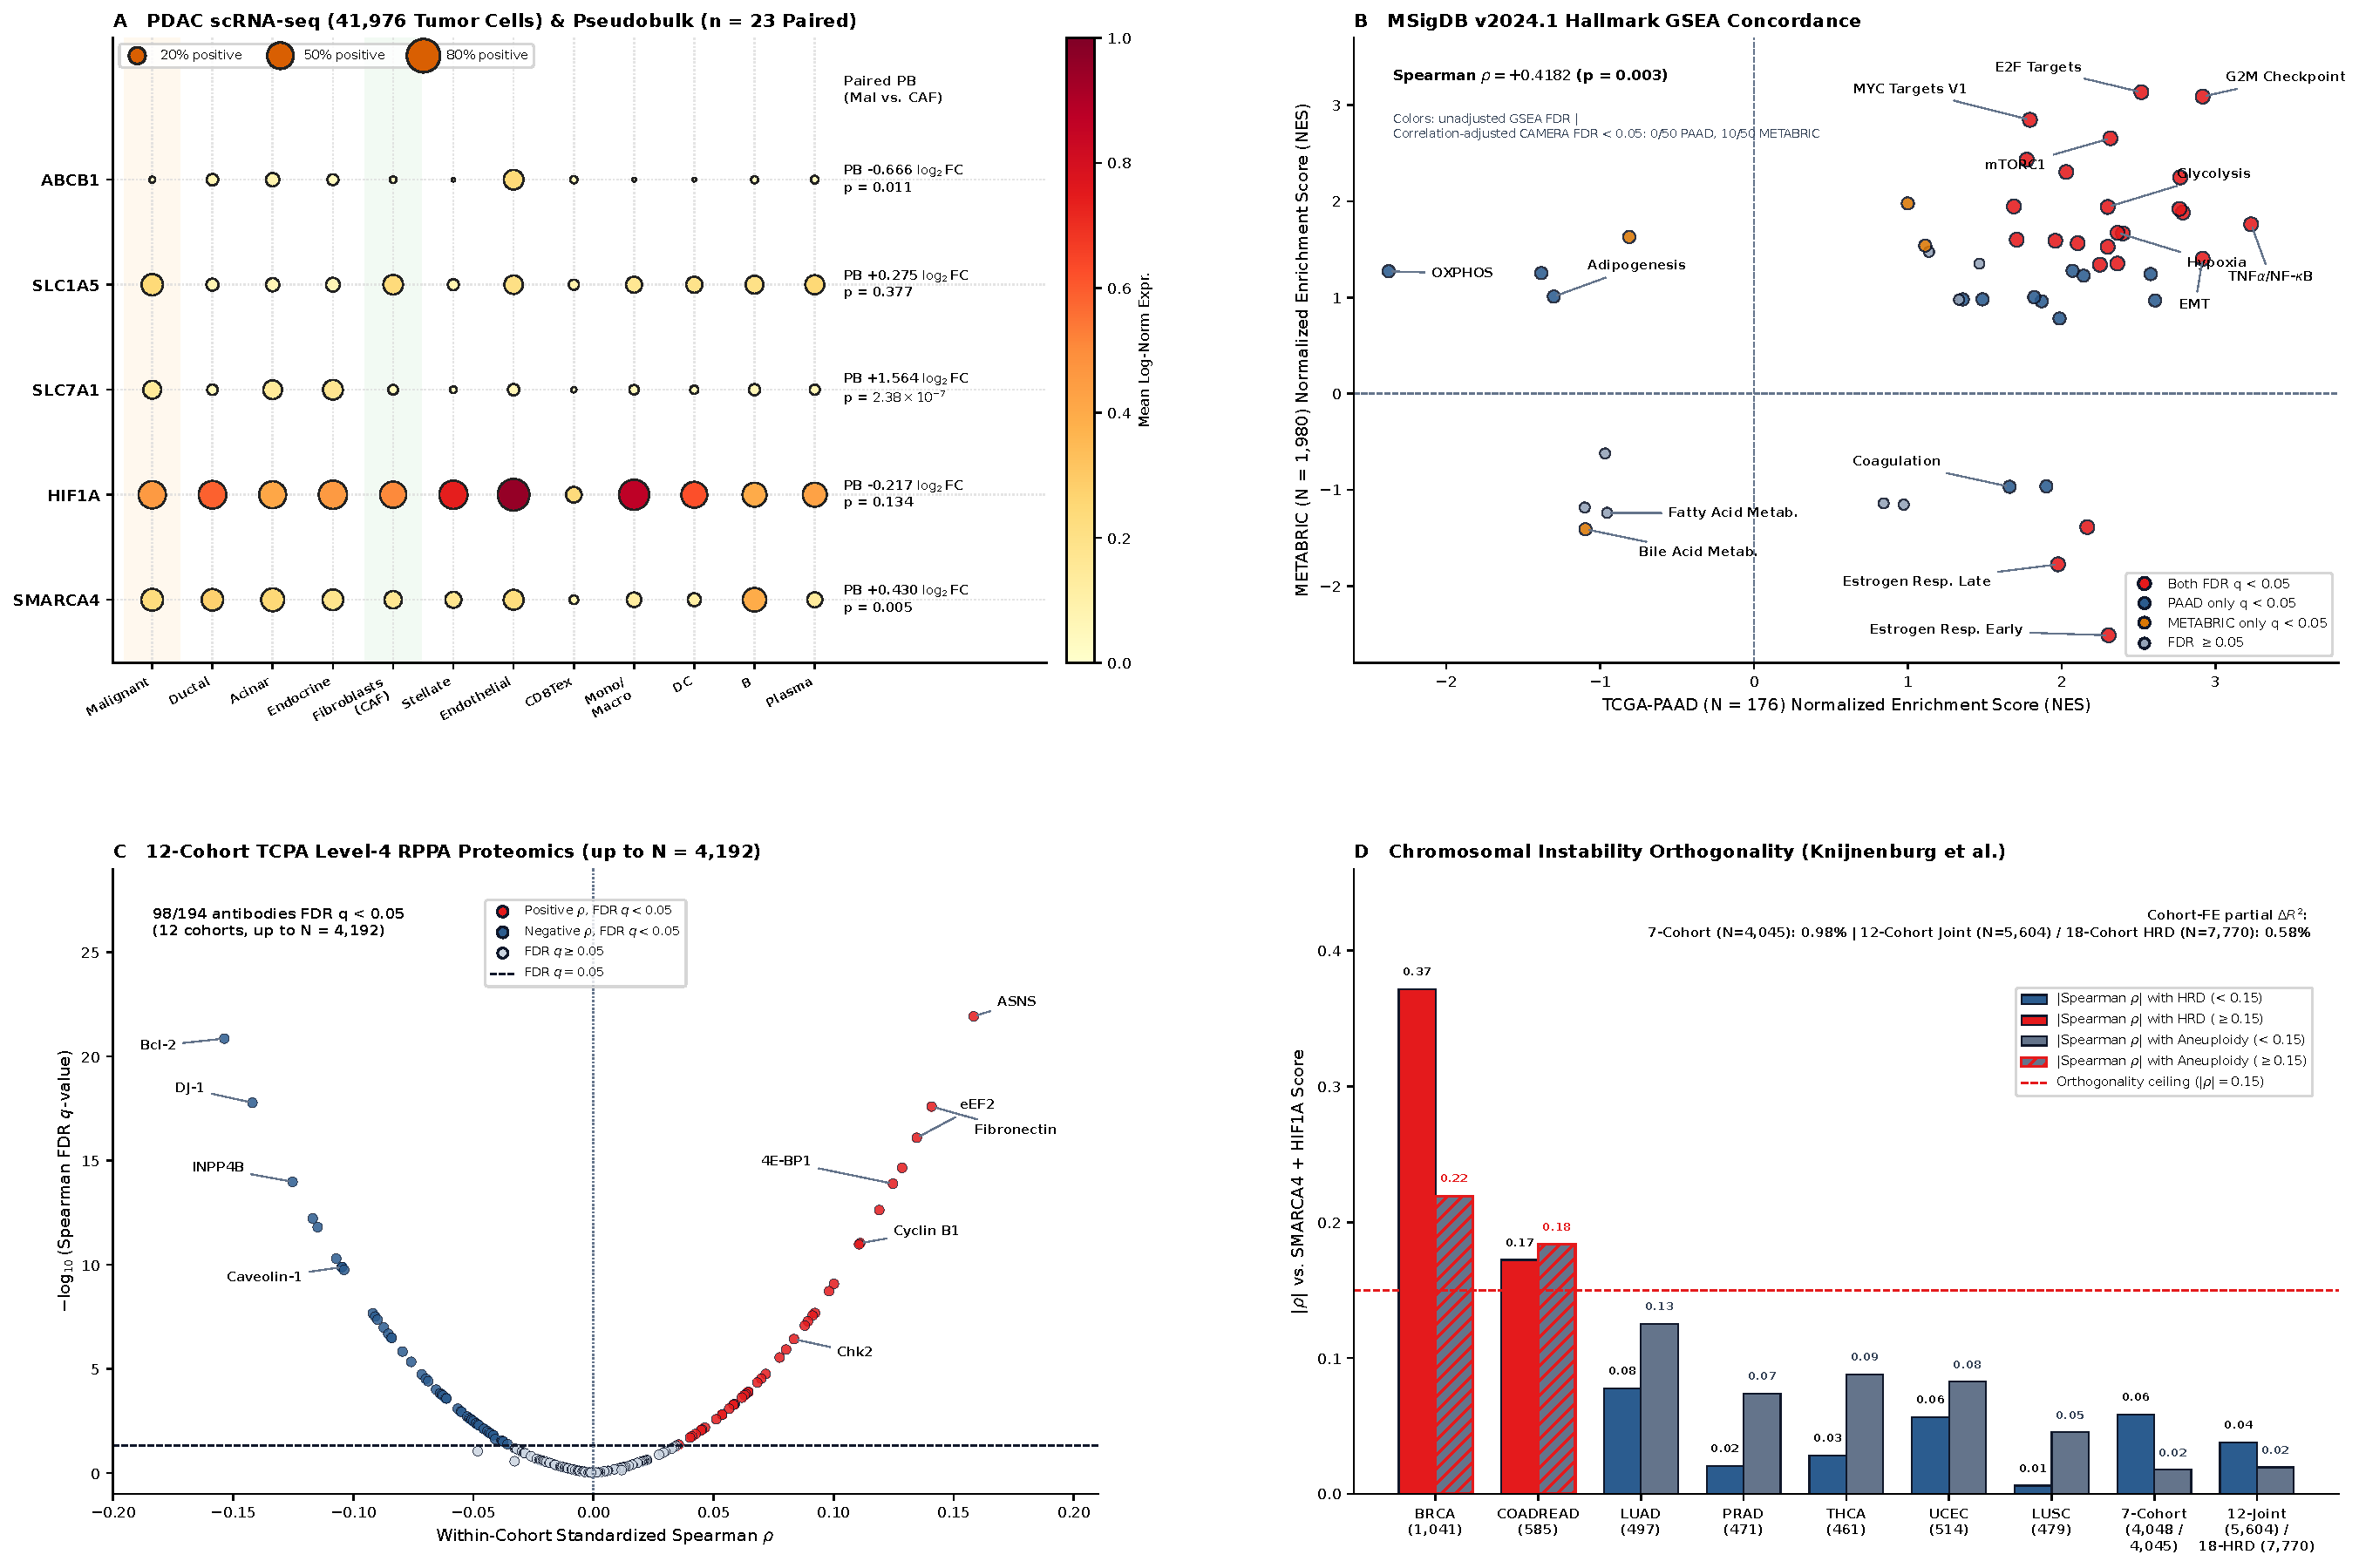
\includegraphics[width=\textwidth]{Figure_4_Final.pdf}
\caption{\textbf{Paired Patient Pseudobulk scRNA-seq Specificity, Hallmark GSEA, Within-Cohort RPPA Proteomics, and Chromosomal Instability Orthogonality.} (A) Patient-level paired pseudobulk comparison ($n = 23$ paired resections, $41,976$ tumor-sample cells within $57,443$ total \texttt{CRA001160} cells) aggregated on single-cell $\exp(y) - 1$ expression, confirming malignant enrichment of \textit{SLC7A1} and \textit{SMARCA4} alongside shared stromal \textit{HIF1A}. (B) MSigDB v2024.1 Hallmark GSEA concordance between primary TCGA-PAAD ($N = 176$) and METABRIC ($N = 1,980$; $\rho = +0.4182$, $p = 0.003$); point colors mark unadjusted GSEA FDR while competitive CAMERA testing yielded $0/50$ sets in TCGA-PAAD and $10/50$ in METABRIC. (C) Cohort-standardized RPPA volcano plot across the 12-cohort TCPA Level-4 compendium (up to $4,192$ patients, $98/194$ antibodies at FDR $q < 0.05$). (D) Cohort-fixed-effect partial $\Delta R^2$ ($0.98\%$ across 7 cohorts, $N = 4,045$ joint; $0.58\%$ across 12 PanCan joint cohorts $N = 5,604$ and 18 HRD cohorts $N = 7,770$) and cohort-level Spearman $|\rho|$ for HRD and aneuploidy scores.}
\label{fig:figure4}
\end{figure*}

\section{Discussion}
Joint analysis of Broad DepMap 24Q2 CRISPR screens, paired hypoxic time-courses, clinical survival cohorts, single-cell PDAC pseudobulk profiles, RPPA proteomics, and GDSC2 drug matrices defines the biological boundaries of the \textit{SMARCA4}--\textit{HIF1A} axis. In normoxic $21\%\ \text{O}_2$ culture, \textit{SLC1A5} and \textit{SLC7A1} show coupled Chronos essentiality across $1,038$ solid tumor lines while non-malignant diploid lines depend less on \textit{SMARCA4}. Yet ambient oxygen tension drives continuous PHD1--3 prolyl hydroxylation and VHL-mediated HIF-1$\alpha$ turnover, breaking \textit{HIF1A}--\textit{SLC7A1} transcriptional coupling relative to $1,384$ primary tumors (Fisher $Z = 6.98$). Only loss-of-function \textit{VHL} mutations ($n = 19$) preserved \textit{HIF1A}--\textit{SLC7A1} Chronos dependency coupling ($r = +0.5412$, $\rho = +0.5439$) alongside selective \textit{EPAS1} vulnerability relative to \textit{VHL}-WT kidney and non-ccRCC lines. Across four NCBI GEO series, $1\%\ \text{O}_2$ hypoxia reliably induced \textit{CA9} and \textit{VEGFA} without raising \textit{HIF1A} mRNA, failed to induce \textit{SLC7A1} in three models, and raised \textit{SLC7A1} only briefly at 24~h in HepG2 before reversing by day~6. In unpaired ChIP-Atlas tracks, strong \textit{SMARCA4} binding in \textit{HIF1A}-null 786-O cells at an intronic \textit{SLC7A1} enhancer occupied by \textit{HIF1A} in RCC4+\textit{VHL} indicates constitutive SWI/SNF bookmarking independent of \textit{HIF1A}. Paired co-ChIP in matched hypoxic cells and physiological 3D models are still needed to test whether \textit{SMARCA4} and HIF-1$\alpha$ assemble cooperatively on that enhancer during prolonged hypoxia.

In patient cohorts, evaluating an unweighted a priori \textit{SMARCA4} + \textit{HIF1A} score prevents overfitting to cohort-specific weights and clarifies where transcriptomic stratification holds. In bulk TCGA-PAAD (median ABSOLUTE purity $0.350$), overall survival is null across full, purity-adjusted, and ductal-restricted models ($p = 0.273\text{--}0.974$), showing that post-translational HIF-1$\alpha$ regulation and tumor heterogeneity limit bulk transcriptomic surrogates. Although paired single-cell profiling detected malignant \textit{SMARCA4} enrichment alongside comparable fibroblast \textit{HIF1A} expression and ICGC/PCAWG-PAAD ($N = 71$) reached significance in age- and sex-adjusted models ($\text{HR} = 1.504$, $p = 0.009$), missing clinical stage data and borderline unadjusted log-rank separation ($p = 0.060$) call for cautious interpretation. Whether opposing malignant effects of \textit{SMARCA4} and hypoxia signaling or stromal composition account for the difference against ICGC/PCAWG-PAAD requires dedicated tumor-intrinsic deconvolution follow-up. Across 10 primary cohorts ($N = 5,102$, $\text{HR}^* = 1.144$) and eight non-breast primary cohorts ($N = 2,586$, $\text{HR}^* = 1.152$), single-gene analysis showed that \textit{SMARCA4} ($\text{HR}^* = 1.153$) drove most of the hazard while \textit{HIF1A} mRNA was null ($\text{HR}^* = 1.047$). Averaging \textit{SMARCA4} with null \textit{HIF1A} compressed between-cohort variance ($I^2 = 16.1\%$) rather than reflecting biological synergy. Adjusting all 10 primary cohorts for \textit{MKI67} proliferation using the full $24,326$-gene CGGA-325 transcriptome attenuated pooled hazard to $\text{HR}^* = 1.084$ ($p = 0.004$) and eliminated glioma risk in CGGA-325 ($\text{HR} = 1.006$, $p = 0.943$; \textit{TOP2A}: $\text{HR} = 0.949$). In BRCA-METABRIC, excluding 513 stage-missing tumors did not bias hazard estimates ($N = 1,979$ $\text{HR} = 1.111$ vs.\ $N = 1,466$ $\text{HR} = 1.115$), and both breast cohorts dropped toward null after adjusting for PAM50 or ER/PR/HER2 status ($\text{HR} = 1.035\text{--}1.070$), matching ER-negative and proliferation signals seen in CAMERA and TCPA RPPA proteomics. Expanding to all 19 solid TCGA cohorts ($N = 7,875$) confirmed a null pan-cancer two-gene hazard ($\text{HR}^* = 1.048$, $p = 0.130$). By contrast, the 14-gene non-cell-cycle \textit{Buffa-14} hypoxia metagene \cite{buffa2010} remained strongly prognostic across all 19 cohorts ($\text{HR}^* = 1.133$, $p = 2.17 \times 10^{-6}$), persisted after \textit{MKI67} control ($\text{HR}^* = 1.116$, $p = 5.54 \times 10^{-7}$, $I^2 = 0.0\%$), and improved nested model fit ($\chi^2_{\text{LRT}}(19) = 56.56$ base; $43.03$ with \textit{MKI67}). True hypoxia transcriptional output therefore drives broad solid-tumor mortality, whereas bulk \textit{HIF1A} mRNA fails as a general proxy and independent \textit{SMARCA4} + \textit{HIF1A} risk after \textit{MKI67} and purity adjustment stays confined to clear cell renal (\texttt{TCGA-KIRC}) and urothelial bladder (\texttt{TCGA-BLCA}) carcinomas.

Normoxic uncoupling similarly limits ambient $21\%\ \text{O}_2$ drug screens. Anchoring GDSC2 monotherapy testing on empirical $1 - \text{AUC}$ avoided $>10\ \mu\text{M}$ curve extrapolations, leaving only Navitoclax at 5\% FDR ($q = 0.049$) and nine compounds at 10\% FDR ($\eta_p^2 = 1.55\%\text{--}2.63\%$), led by BH3-mimetics, platinum agents, Entinostat, and Uprosertib. All nine kept significance under \textit{MKI67} control, whereas TOP1 and PARP1/2 trends weakened once proliferation was accounted for, and $0/3$ tested combinations tracked baseline risk after lineage adjustment. Instead, response followed established downstream gates, \textit{SLFN11} and \textit{BAK1}, across both $1 - \text{AUC}$ and $\ln(\text{IC}_{50})$. Because Phase~I AZD5991 trials reported dose-limiting troponin elevations \cite{desai2024}, our harmonized UCSC Xena Toil comparisons against GTEx v6 provide critical safety context: normal Heart Left Ventricle ($44.08$ TPM), Heart Atrial Appendage ($59.22$ TPM), and Liver ($67.54$ TPM) express substantial \textit{MCL1}, and Whole Blood ($135.67$ TPM) exceeds solid tumors ($114.25$ TPM), while \textit{BRD4} shows narrow tumor margins ($1.45\times\text{--}1.90\times$). Together with flat GDSC2 $1 - \text{AUC}$ curves for single-agent AZD5991 ($0.0309$) and Olaparib ($0.0407$) and missing public human AZD5991 $C_{\max}$, plasma $f_u$, and raw $7 \times 7$ viability matrices, these results favor tumor-targeted delivery, iPSC-cardiomyocyte toxicity counter-screens, \textit{BAK1}/\textit{SLFN11} patient selection, and $1\%\ \text{O}_2$ 3D organoid testing while systemic dose-sparing remains unverified.

\section{Methods}

\subsection{DepMap 24Q2 Functional Genomics, Co-Essentiality, and Uncoupling}
CRISPR-Cas9 Chronos gene effect scores, $\log_2(\text{TPM}+1)$ RNA-seq profiles ($1,719$ unique default models across $1,775$ profiles), cell line annotations, and somatic mutation calls were obtained from Broad DepMap Public 24Q2 \cite{depmap2021}. Excluding hematopoietic and non-cancerous models yielded $1,038$ solid tumor CRISPR lines and 16 non-malignant diploid controls, with paralog specificity assessed across $1,186$ CRISPR-screened lines. For \textit{SMARCA4} co-essentiality, solid lines were stratified into \textit{SMARCA4}-dependent ($\text{Chronos} \le -0.50$, $n = 299$) and independent ($\text{Chronos} \ge -0.10$, $n = 251$) groups and tested across $18,434$ genes using two-sided Welch's $t$-tests with Benjamini-Hochberg FDR control alongside continuous Pearson and Spearman correlations across all $1,038$ solid lines.

Complete-case cBioPortal PanCancer $\log_2(\text{RSEM}+1)$ expression matrices across TCGA-PAAD ($n = 176$), TCGA-GBM ($n = 158$), and TCGA-BRCA ($n = 1,050$) totaling $N = 1,384$ primary tumors were compared against within-lineage Z-scored unique solid DepMap lines ($n = 1,349$), unadjusted DepMap models ($1,719$ unique / $1,775$ profiles), and Pancreas/CNS/Breast models ($n = 229$ unique; $n = 221$ solid-filtered) using Fisher's $r$-to-$z$ test. \textit{VHL} mutations were restricted to predicted loss-of-function, damaging, truncating, or splice variants, comparing 19 \textit{VHL}-LoF lines against $1,019$ wild-type solid lines, 15 wild-type kidney lines, $1,004$ non-kidney lines, and $1,018$ non-ccRCC wild-type lines using Pearson correlation, Spearman correlation, 19-fold leave-one-out deletion (range $r = +0.4706$ to $+0.6274$, all $p < 0.05$), Cohen's $d$, and two-sided Welch's $t$-tests on \textit{EPAS1}.

Direct hypoxic transcriptomic responses were tested across four public NCBI GEO $1\%$ versus $21\%\ \text{O}_2$ solid-tumor series: \texttt{GSE283995} (HepG2 RNA-seq: normoxia $n = 6$, 24~h $n = 6$, and day-6 chronic hypoxia $n = 5$; Welch's $t$-test), \texttt{GSE139673} (AsPC-1 $\log_2(\text{CPM}+1)$, $n = 3$ pairs in control and \textit{siARNT} arms; paired $t$-test), \texttt{GSE145108} (RKO, A549, and H460 $\log_2(\text{RPKM}+1)$, evaluated pooled across $n = 6$ pairs and per line at $n = 2$ pairs; paired $t$-test), and \texttt{GSE300765} (U87MG Illumina HumanHT-12 v4 BeadChip \texttt{GPL10558}, $n = 3$ pairs; paired $t$-test). Unpaired solid-tumor ChIP-seq peak overlaps at \textit{SLC7A1} (\texttt{chr13:29,500,000--29,620,000}) and \textit{VEGFA} (\texttt{chr6:43,760,000--43,790,000}, GRCh38/hg38) used MACS2 $q < 10^{-5}$ BED calls from nine ChIP-Atlas tracks (\textit{HIF1A}: \texttt{SRX15691692}, \texttt{SRX666556}, \texttt{SRX2584127}, \texttt{SRX3342251}; \textit{SMARCA4}: \texttt{SRX8566545}, \texttt{SRX1156541}, \texttt{SRX1156535}, \texttt{SRX10640844}, \texttt{SRX6743053}).

\subsection{Unweighted A Priori Score, Clinical Survival, and Meta-Analysis}
Primary TCGA-PAAD survival modeling used PanCancer Atlas primary tumor RNA-seq profiles ($N = 176$, 92 deaths) merged with PanCanAtlas ABSOLUTE purity (median $0.350$) and the Raphael et al.\ ductal PDAC whitelist ($N = 148$ complete) \cite{raphael2017}. Our 10-cohort primary survival panel ($N = 5,102$, $2,162$ deaths; Table~1) paired eight initial TCGA cohorts---selected by combining our focal PDAC cohort (\texttt{TCGA-PAAD}) with high-mortality cBioPortal solid-tumor archives (\texttt{BLCA}, \texttt{GBM}, \texttt{KIRC}, \texttt{LIHC}, \texttt{SKCM}) and large representative PanCancer Atlas studies (\texttt{BRCA}, \texttt{SARC})---with the non-TCGA BRCA-METABRIC \cite{curtis2012} and CGGA-325 \cite{cgga2021} cohorts. To prevent cohort-selection bias, we evaluated all 19 adult solid TCGA cohorts having complete survival, stage or grade, and RNA-seq RSEM data ($N = 7,875$, $2,362$ deaths; adding \texttt{LUAD}, \texttt{LUSC}, \texttt{COADREAD}, \texttt{HNSC}, \texttt{STAD}, \texttt{OV}, \texttt{UCEC}, \texttt{CESC}, \texttt{ESCA}, \texttt{THCA}, and \texttt{PRAD}) as a co-primary pan-cancer benchmark alongside the 10-cohort panel; the remaining nine rarer TCGA tumor types (\texttt{KIRP}, \texttt{KICH}, \texttt{MESO}, \texttt{UCS}, \texttt{UVM}, \texttt{ACC}, \texttt{CHOL}, \texttt{PCPG}, and \texttt{TGCT}) lacked paired PanCancer Atlas clinical and RSEM archives in the public download set. Survival modeling across every cohort used the unweighted a priori two-gene score $Z(z_{\textit{SMARCA4}} + z_{\textit{HIF1A}})$ standardized within each cohort to mean 0 and SD 1. Multivariable Cox models adjusted for available clinical covariates: age, clinical stage or histological grade (\texttt{UCEC} and \texttt{CESC} used grade; \texttt{PRAD}, \texttt{SARC}, and \texttt{GBM} used age), ABSOLUTE purity in TCGA-PAAD (and sensitivity models in TCGA-KIRC and TCGA-BLCA), IDH mutation and MGMT methylation in CGGA-325, and age plus sex in ICGC/PCAWG-PAAD ($N = 71$, 48 deaths; stage and purity unavailable).

Proportional hazards assumptions were tested across all 22 cohorts (10 primary, ICGC/PCAWG-PAAD, and 11 additional TCGA cohorts) via Schoenfeld residuals on rank-transformed survival time. Proliferation-adjusted sensitivity models added standardized \textit{MKI67} across all eight primary TCGA cohorts ($N = 3,323$), BRCA-METABRIC ($N = 1,466$), the full $24,326$-gene public CGGA-325 RSEM matrix \cite{cgga2021} ($N = 313$, evaluated using $\log_2(\text{RSEM}+1)$ [$\text{HR} = 1.006$, $p = 0.943$] and linear RSEM \textit{MKI67} [$\text{HR} = 1.010$, $p = 0.894$] alongside \textit{TOP2A}), and all 19 solid TCGA cohorts ($N = 7,875$). In BRCA-METABRIC, we compared all $1,979$ complete-OS cases adjusted for age against the $1,466$ stage-complete subset to rule out selection bias from 513 stage-missing tumors, and further adjusted complete cases for PAM50/Claudin-low ($N = 1,463$) and ER/PR/HER2 receptor status ($N = 1,466$), mirroring PAM50 adjustment in TCGA-BRCA ($N = 950$). To benchmark transcriptional hypoxia activity across all 19 solid TCGA cohorts ($N = 7,875$), we excluded cell-cycle \textit{CDKN3} from the 15-gene Buffa metagene \cite{buffa2010}, averaged within-cohort Z-scores of the remaining 14 core hypoxia genes (\textit{ACOT7}, \textit{ADM}, \textit{ALDOA}, \textit{ENO1}, \textit{LDHA}, \textit{MIF}, \textit{MRPS17}, \textit{NDRG1}, \textit{P4HA1}, \textit{PGAM1}, \textit{SLC2A1}, \textit{TPI1}, \textit{TUBB6}, and \textit{VEGFA}), and compared \textit{Buffa-14} and \textit{SMARCA4} + \textit{Buffa-14} against \textit{SMARCA4} + \textit{HIF1A} using DerSimonian-Laird random-effects pooling, summed nested likelihood-ratio tests ($\text{df} = 19$), and $N$-weighted mean C-index differences.

\subsection{Lineage-Controlled Type II ANOVA, Bliss Synergy, and Toil Comparisons}
Full-screen monotherapy Type~II ANOVA evaluated $m = 286$ compounds in Sanger GDSC2 across solid-tumor cell lines spanning 19--24 tissue lineages. DepMap \textit{SMARCA4}, \textit{HIF1A}, and \textit{MKI67} RNA-seq values were standardized within malignant solid lines before regressing empirical $1 - \text{AUC}$ (bounded $[0, 1]$ to avoid $>10\ \mu\text{M}$ curve-fit extrapolations) on the baseline risk score and tissue lineage fixed effects, reporting partial $R^2$ ($\eta_p^2 = \text{SS}_{\text{risk}} / (\text{SS}_{\text{risk}} + \text{SS}_{\text{resid}})$), \textit{MKI67}-adjusted models, and secondary $\ln(\text{IC}_{50})$ concordance checks. Combination screens pooled $84,055$ matrix rows ($69,121$ solid rows) across five Sanger GDSC combination matrices (\texttt{gdsc-007}--\texttt{gdsc-010} and \texttt{sandpiper-01}) \cite{jaaks2022,bashi2024}, collapsing replicate peak $3 \times 3$ Bliss windows per unique cell line against the 109-pair background median ($+0.0662$) via two-sided Wilcoxon signed-rank tests. Monotherapy gates (\textit{SLFN11}, \textit{BAK1}, \textit{BAX}) were tested on empirical $1 - \text{AUC}$ and $\ln(\text{IC}_{50})$ using raw Pearson correlation, lineage-residualized partial correlation ($\text{df} = n - L - 1$), and two-sided Mann-Whitney $U$ tests.

For the normal-organ safety comparison, we queried the harmonized UCSC Xena Toil RNA-seq recompute hub (\texttt{TcgaTargetGtex\_rsem\_gene\_tpm}, unit $\log_2(\text{TPM}+0.001)$ back-transformed via $2^y - 0.001$) \cite{vivian2017} for \textit{MCL1}, \textit{BAK1}, \textit{BRD4}, and \textit{SMARCA4} across $n = 9,138$ TCGA primary solid tumors (excluding hematologic malignancies) and GTEx v6 normal Heart Left Ventricle ($n = 202$), Heart Atrial Appendage ($n = 175$), Liver ($n = 110$), and Whole Blood ($n = 337$), noting that Whole Blood transcripts remain globally diluted by erythrocyte globin mRNA. Matrix \texttt{D1} anchors and extrapolated $\text{IC}_{50}$ medians from combination summaries were compared against GDSC2 $1 - \text{AUC}$ distributions, screening ceilings ($10\ \mu\text{M}$ max in GDSC2 for AZD5153, AZD5991, and Olaparib; $10\text{ nM}$ in GDSC2 and $300\text{ nM}$ in combinations for SN-38), and published Phase~I AZD5153 total plasma $C_{\max}$ values \cite{hamilton2023}. Because numerical AZD5991 $C_{\max}$ \cite{desai2024}, human plasma unbound fractions ($f_u$) \cite{tron2018}, and per-well $7 \times 7$ viability curves are absent from public releases, Chou-Talalay $\text{DRI}$ and unbound $C_{\max, u}$ models were omitted.

\subsection{Pseudobulk scRNA-seq, Pathway Analysis, RPPA Proteomics, and Chromosomal Instability}
Single-cell count matrices from \texttt{CRA001160} ($57,443$ quality-controlled cells; $41,976$ tumor-sample cells across 24 PDAC patients) \cite{peng2019} were analyzed with TISCH2 annotations \cite{han2023}. Inspection across all $142,020,944$ nonzero entries in the HDF5 archive confirmed natural-log $\ln(\text{CP10K}+1)$ scaling ($\min = 0.0905$, median $= 0.9679$, $\max = 8.9038$). Single-cell values were therefore back-transformed via $\exp(y) - 1$ before patient- and cell-type averaging across $n = 23$ paired resections, testing differential abundance via $\log_2((\overline{\text{Mal}}_p + 0.01)/(\overline{\text{CAF}}_p + 0.01))$ and two-sided paired Wilcoxon tests. Pathway enrichment across 50 MSigDB v2024.1 Hallmark gene sets \cite{liberzon2015} used the unweighted two-gene median split in primary TCGA-PAAD ($N = 176$) and METABRIC ($N = 1,980$) via pre-ranked GSEA on Welch's $t$-statistics ($1,000$ permutations) alongside Wu--Smyth competitive CAMERA tests \cite{wu2012}. Cohort-standardized 12-cohort TCPA Level-4 RPPA proteomics ($4,192$ patients) \cite{li2013,akbani2014}, cohort-fixed-effect chromosomal instability OLS models across seven ($N = 4,045$ joint) and extended TCGA cohorts ($N = 5,604$ joint across 12 PanCan cohorts; $N = 7,770$ HRD across 18 cohorts) \cite{knijnenburg2018}, and IMvigor210 survival ($N = 347$) \cite{mariathasan2018} were all evaluated on the identical unweighted two-gene score.

\vspace{-4pt}
\section*{Data and Code Availability}
\vspace{-3pt}
{\raggedright Source scripts, processed tables, and figure pipelines are archived at \url{https://github.com/SachsinSinnathurai/smarca4-hif1a-pharmacogenomics}. Public datasets derive from Broad DepMap 24Q2, TCGA PanCancer Atlas, METABRIC, full-transcriptome CGGA-325 (\texttt{cgga.org.cn}), Sanger GDSC2/Combinations, TCPA, TISCH2 (\texttt{CRA001160}), IMvigor210, UCSC Xena Toil (TCGA vs.\ GTEx v6, \texttt{toil.xenahubs.net}), NCBI GEO (\texttt{GSE283995}, \texttt{GSE139673}, \texttt{GSE145108}, \texttt{GSE300765}), and ChIP-Atlas.\par}

\vspace{-6pt}
\section*{Conflict of Interest Statement}
\vspace{-3pt}
The author declares no competing financial interests.

\vspace{-6pt}
\section*{Author Contributions}
\vspace{-3pt}
S.S. conceived the study, designed the analytical pipelines, executed all statistical and bioinformatics analyses, interpreted the data, and wrote the manuscript.

\vspace{-6pt}
\section*{Funding Statement}
\vspace{-3pt}
This research was conducted independently by the author without external grant funding.

\section*{AI Assistance Statement}
Large language model tools were used strictly as coding assistants for Python and LaTeX scripting boilerplate, syntax debugging, and pipeline formatting. All biological hypotheses, statistical models, dataset integrations, numerical verifications, and manuscript writing were performed by the author.

\vspace{-5pt}
\begingroup
\footnotesize
\begin{thebibliography}{24}
\setlength{\itemsep}{1pt}
\setlength{\parskip}{0pt}
\bibitem{depmap2021} Dempster, J. M., et al. (2021). Chronos: a cell population dynamics model of CRISPR experiments that improves inference of gene fitness effects. \textit{Genome Biology}, 22(1), 343.
\bibitem{ivan2001} Ivan, M., et al. (2001). HIF$\alpha$ targeted for VHL-mediated destruction by proline hydroxylation: implications for O$_2$ sensing. \textit{Science}, 292(5516), 464--468.
\bibitem{jaakkola2001} Jaakkola, P., et al. (2001). Targeting of HIF-$\alpha$ to the von Hippel-Lindau ubiquitylation complex by O$_2$-regulated prolyl hydroxylation. \textit{Science}, 292(5516), 468--472.
\bibitem{kenneth2009} Kenneth, N. S., Mudie, S., van Uden, P., \& Rocha, S. (2009). SWI/SNF regulates the cellular response to hypoxia. \textit{Journal of Biological Chemistry}, 284(7), 4123--4131.
\bibitem{sena2013} Sena, J. A., Wang, L., \& Hu, C.-J. (2013). BRG1 and BRM chromatin-remodeling complexes regulate the hypoxia response by acting as coactivators for a subset of hypoxia-inducible transcription factor target genes. \textit{Molecular and Cellular Biology}, 33(19), 3849--3863.
\bibitem{tcga2018} Liu, J., et al. (2018). An Integrated TCGA Pan-Cancer Clinical Data Resource to Drive High-Quality Survival Outcome Analytics. \textit{Cell}, 173(2), 400--416.
\bibitem{raphael2017} Raphael, B. J., et al. (2017). Integrated Genomic Characterization of Pancreatic Ductal Adenocarcinoma. \textit{Cancer Cell}, 32(2), 185--203.
\bibitem{buffa2010} Buffa, F. M., Harris, A. L., West, C. M., \& Miller, C. J. (2010). Large meta-analysis of multiple cancers reveals a common, compact and highly prognostic hypoxia metagene. \textit{British Journal of Cancer}, 102(2), 428--435.
\bibitem{jaaks2022} Jaaks, P., et al. (2022). Effective drug combinations in breast, colon and pancreatic cancer cells. \textit{Nature}, 603(7899), 166--173.
\bibitem{bashi2024} Bashi, A. C., et al. (2024). Large-scale pan-cancer cell line screening identifies actionable and effective drug combinations. \textit{Cancer Discovery}, 14(5), 846--865.
\bibitem{cgga2021} Zhao, Z., et al. (2021). Chinese Glioma Genome Atlas (CGGA): A Comprehensive Resource with Functional Genomic Data from Chinese Glioma Patients. \textit{Genomics, Proteomics \& Bioinformatics}, 19(1), 1--12.
\bibitem{curtis2012} Curtis, C., et al. (2012). The genomic and transcriptomic architecture of 2,000 breast tumours reveals novel subgroups. \textit{Nature}, 486(7403), 346--352.
\bibitem{peng2019} Peng, J., et al. (2019). Single-cell RNA-seq highlights intra-tumoral heterogeneity and malignant progression in pancreatic ductal adenocarcinoma. \textit{Cell Research}, 29(9), 725--738.
\bibitem{han2023} Han, Y., et al. (2023). TISCH2: expanded datasets and new tools for single-cell transcriptome analyses of the tumor microenvironment. \textit{Nucleic Acids Research}, 51(D1), D1425--D1431.
\bibitem{liberzon2015} Liberzon, A., et al. (2015). The Molecular Signatures Database (MSigDB) hallmark gene set collection. \textit{Cell Systems}, 1(6), 417--425.
\bibitem{wu2012} Wu, D., \& Smyth, G. K. (2012). Camera: a competitive gene set test accounting for inter-gene correlation. \textit{Nucleic Acids Research}, 40(17), e133.
\bibitem{li2013} Li, J., et al. (2013). TCPA: a resource for cancer functional proteomics data. \textit{Nature Methods}, 10(11), 1046--1047.
\bibitem{akbani2014} Akbani, R., et al. (2014). A pan-cancer proteomic perspective on The Cancer Genome Atlas. \textit{Nature Communications}, 5, 3887.
\bibitem{knijnenburg2018} Knijnenburg, T. A., et al. (2018). Genomic and molecular landscape of DNA damage repair deficiency across The Cancer Genome Atlas. \textit{Cell Reports}, 23(1), 239--254.
\bibitem{mariathasan2018} Mariathasan, S., et al. (2018). TGF-$\beta$ attenuates tumour response to PD-L1 blockade by contributing to exclusion of T cells. \textit{Nature}, 554(7693), 544--548.
\bibitem{vivian2017} Vivian, J., et al. (2017). Toil enables reproducible, open source, big biomedical data analyses. \textit{Nature Biotechnology}, 35(4), 314--316.
\bibitem{desai2024} Desai, P., et al. (2024). A Phase 1 First-in-Human Study of the MCL-1 Inhibitor AZD5991 in Patients with Relapsed/Refractory Hematologic Malignancies. \textit{Clinical Cancer Research}, 30(21), 4844--4855.
\bibitem{hamilton2023} Hamilton, E. P., et al. (2023). First-in-human Study of AZD5153, A Small-molecule Inhibitor of Bromodomain Protein 4, in Patients with Relapsed/Refractory Malignant Solid Tumors and Lymphoma. \textit{Molecular Cancer Therapeutics}, 22(10), 1154--1165.
\bibitem{tron2018} Tron, A. E., et al. (2018). Discovery of Mcl-1-specific inhibitor AZD5991 and preclinical activity in multiple myeloma and acute myeloid leukemia. \textit{Nature Communications}, 9(1), 5341.
\end{thebibliography}
\endgroup
\end{document}
